\documentclass[12pt,letterpaper]{report}

\usepackage{cite}
\usepackage{amssymb}
\usepackage{amsmath}
\usepackage{accents}
\usepackage{qtree}
\usepackage{xkeyval}
\usepackage{graphicx}
\usepackage{amsfonts}
\usepackage[greek,english]{babel}
\usepackage[T1]{fontenc}

\begin{document}
\newcommand{\double}{\par\setlength{\baselineskip}{22pt}}

\providecommand{\abs}[1]{\left\lvert#1\right\rvert}
\providecommand{\norm}[1]{\left\lVert#1\right\rVert}

\pagestyle{plain}

\title{Diaplexis: A C++ Library for Combinatorial Spacetime Models}
\author{Daniel Stubbs}

\maketitle

\newpage

\double

\chapter{Introduction}

This document will discuss the structure and use of the Diaplexis library, a set of C++ 
classes and functions for investigating combinatorial spacetime models. It corresponds 
to version 1.0 of the Diaplexis library, released on \today.  

The Diaplexis library's principal class is \texttt{Spacetime} which depends however on a 
large collection of auxiliary classes, some from the Synarmosma library, with the entire 
hierarchy illustrated in Figure \ref{fig:class_hierarchy}. 
\begin{figure}[htb]
\centering
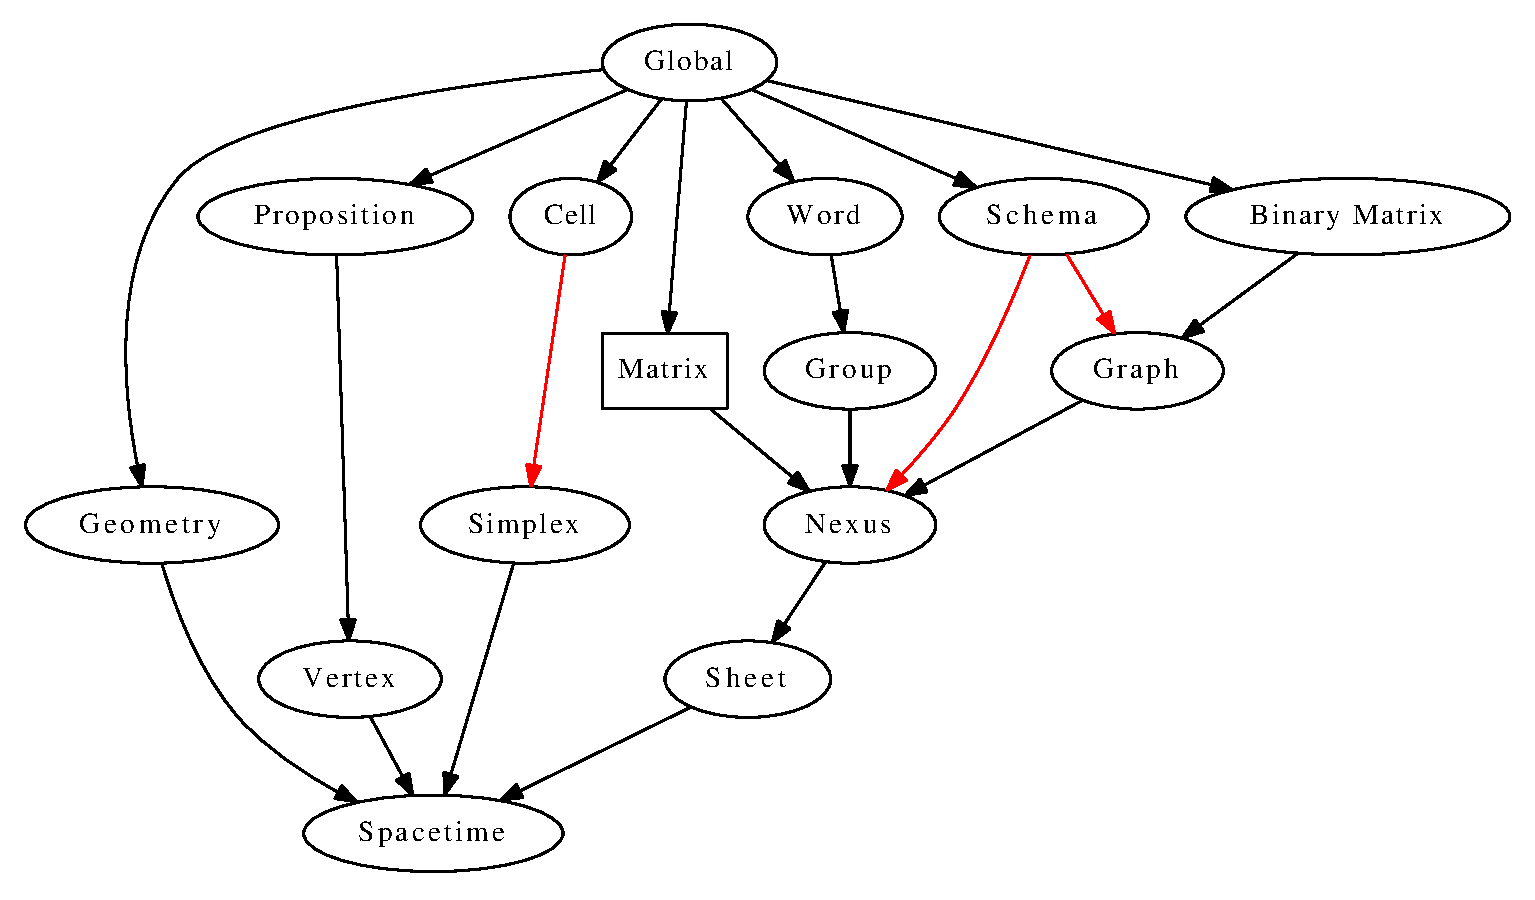
\includegraphics[width=4in]{images/class_hierarchy.eps}
\caption{Diaplexis Class Diagram (black indicates composition, red inheritance and a 
class in green comes from the Synarmosma library)}
\label{fig:class_hierarchy}
\end{figure}
A user can either make use of the \texttt{Spacetime} as it is or else derive a further class 
from it, replacing certain methods with ones that better reflect the spacetime structure of 
a given alternative model. 

The ubiquity of a $d$-simplex $\Sigma$ is represented as either an STL vector $\mathbf{v}$ of integers 
whose length is equal to the number of sheets $N$ in the spacetime complex, where $v_k=0$ or 
$1$ distinguishes whether $S$ is a member of the $k$-th sheet, or an instance $\chi$ of the 
class NTL::ZZ. In the latter case, each sheet is assigned a colour $p_k$ which is a prime number 
and $\chi$ is then the product of all the colours of the sheets of which it is a member so that 
membership is tested by divisibility $p_k \mid \chi$ implies that $S$ is a member of the $k$-th 
sheet. 

The program begins with the spacetime complex in a given initial state and then seeks to 
evolve it through a relaxation process to an asymptotic state where the total error in the 
structure equation for the spacetime complex is less than some cutoff, $\varepsilon = 10^{-6}$ 
for example. This adaptation process normally involves both significant topological and 
geometric changes, the two being intimately linked with the spacetime's energy distribution 
through the aforementioned structure equation. The energy distribution arises from the 
\texttt{Vertex} class, which has a property \texttt{energy} represented by a double precision 
number, subject to the restriction that the energy is always greater than or equal to zero. 
It is the energy distribution which is the motor of topological entwinement and geometric 
curvature in the combinational spacetime model that is at the heart of the Diaplexis library.  

\section{Compilation and Installation}

Compiling the Diaplexis library requires a modern C++ compiler (g++, icpc etc.) as well as 
the Boost System and Thread libraries, the Number Theory Library (NTL), the BLAS/LAPACK 
libraries and the PugiXML library for XML processing. Once the diaplexis-latest.tar.gz file is 
obtained from www.synarmosma.org/downloads you can untar it via the command\newline
\texttt{tar -xzf diaplexis-latest.tar.gz}\newline
then change directory,\newline
\texttt{cd diaplexis/src}\newline  
and finally type the command \texttt{make install} to begin the build process. Once this is 
complete, you can decide whether to use the NTL or STL version of the simplicial ubiquity 
as the default and use the script command \texttt{./set\_default} with the argument NTL or STL 
to make the necessary changes. The compilation of the Diaplexis library has been 
tested on several Unix platforms, including OS X (10.9 on Intel) and Linux on the x86, 
x86-64, IA-64 and ARM architectures, using both the g++ and icpc compilers. In principle it 
should also run under Windows using the Cygwin environment. 

Normally the only file that a user should need to modify in order to build the Diaplexis library 
is \texttt{Makefile.def}, where various compiler arguments and libraries are all specified. Note that 
the build process expects the compiler to be defined in the environment variable \texttt{CXX}, along 
with the existence of the environment variables \texttt{CXX\_FLAGS}, \texttt{CXX\_OPT} and \texttt{DEBUG}. 
The two final variables \texttt{CXX\_OPT} and \texttt{DEBUG} control the compilation flags used for 
optimization and debugging. Typical values for these two environment variables would be (for the Gnu 
C++ compiler on the x86-64/Linux platform) \texttt{-O3 -march=native -fstrict-aliasing -funroll-loops} 
and \texttt{-g}.

In general the default values for the optimization level in this file can be used as 
they should be safe. The only changes to the source code that would normally be of interest 
concern the value of certain global constants. These constants are summarized in the following table,
\begin{table}[htbp]
\centering
\begin{tabular}{|c|c|c|c|}
\hline
\emph{Constant Name} & \emph{Quantity Represented} & \emph{Type} & \emph{Scope} \\ \hline
\texttt{ND} & Maximum Dimension of                  & \texttt{int} & Global \\ 
           & Spacetime Complex                     &             &        \\ \hline
\texttt{NP} & Number of Atomic                       & \texttt{int} & Global \\ 
           & Propositions per Clause               &              &         \\ \hline
\texttt{background\_dimension} & Spacetime Dimension far & \texttt{int}  & Geometry \\ 
                              & from an Energy Source    &             &           \\ \hline
\texttt{topological\_radius} & Combinatorial Radius & \texttt{int} & Spacetime \\
                            & for Graph Capture &          &           \\ \hline
\texttt{ramosity} & Polycosmic Branching & \texttt{double} & Spacetime \\ \hline
\texttt{epsilon} & Convergence Criterion & \texttt{double} & Spacetime \\ \hline
\texttt{T\_zero} & Initial Temperature for & \texttt{double} & Spacetime \\
               & Permutation Annealing   &                &           \\ \hline
\texttt{kappa} & Thermal Decay Rate for   & \texttt{double} & Spacetime \\
              & Permutation Annealing    &                &           \\ \hline
\end{tabular}
\caption{Compile-Time Parameters}
\label{ct_parms}
\end{table}
There are four conditional compilation parameters which could be useful to alter, 
\texttt{FLAT}, \texttt{VERBOSE}, \texttt{PARALLEL} and \texttt{LEIBNIZ}. The effect of the 
first is to control how the geometric distance between two vertices is calculated; 
if the library is compiled with this option, then the geometric difference between 
two vertices will always be calculated as if both vertices had the same dimension, 
equal to the value \texttt{background\_dimension}. Otherwise the difference calculated 
will be a vector of length equal to the greatest dimension of the two vertices and 
if not the same for both vertices, the lower dimensional one will have values close 
to zero assigned to its coordinate vector for the missing dimensions. 

The \texttt{VERBOSE} flag causes the Diaplexis library to write a great deal of 
diagnostic logging information to the standard output during execution and is normally 
only useful for developers. That said, with this flag users can have access to a 
wealth of information about the library's reasoning process for the hyphantic operators 
that are used, information which does not appear in the log file created by the normal 
execution of the library. The quantity of text generated by this flag is sufficiently 
large however that users should redirect the standard output to a disk file for subsequent 
analysis. 

The flag \texttt{PARALLEL} causes the library to be compiled with OpenMP directives to 
parallelize certain time-consuming loops and regions of the library; its use supposes the 
existence of a C++ compiler that supports OpenMP 3.1. 

Finally, the \texttt{LEIBNIZ} flag\footnote{Named in honour of the German philosopher and 
mathematician Gottfried Wilhelm Leibniz (1646--1716), whose writings contain the first 
modern discussion of such a model of geometry in opposition to the ``absolute'' model that 
was pioneered by Descartes in 1637 and used so effectively by Newton in the development of 
his mechanics.} has a fairly radical effect on the codebase as it attempts to employ a purely 
relational model for the spacetime geometry. When it is present during the compilation, the 
Geometry class has its coordinates property replaced by a hash table that maps a string 
``u:v'' to an index in the vector distances. This relational geometry consists then of the 
set of all $n(n-1)/2$ distances between the $n$ vertices in the spacetime complex, without 
however any angular data. For those parts of the program that absolutely require the 
existence of coordinates (such as the visualization methods) there is a method of the Geometry 
class which uses the symmetric distance matrix $\Delta$ to compute a possible embedding in 
$\mathbb{R}^D$ by means of the metric multi-dimensional scaling (MDS) technique that is widely 
used in statistics.   
%When it is used, the property \texttt{Vertex::x} is replaced by a set of angles $\{\theta_i\}$, 
%drawn from a parameterization of the Lie group $\text{SO}(n,\mathbb{R})$ where $n$ has the 
%value of \texttt{background_dimension}. The other fundamental geometric variable is the 
%set of lengths of 1-simplices $\ell_i$. If the spacetime complex's background dimension 
%is two this operation is relatively straightforward but when it is greater than two, 
%the parameterization of $\text{SO}(n,\mathbb{R})$ is non-trivial for $n>2$. In addition, 
%there are many routines in the Diaplexis library that presuppose the ease of calculating 
%the distance between any two vertices $u$ and $v$, which in the relational model is by 
%no means evident though if they share a common neighbour we can use the triangle 
%inequality to construct an upper bound on their mutual distance.  

\section{Basic Usage}

As the simplest possible example of the use of the Diaplexis library, we consider the 
following content,
\begin{verbatim}
#include "diaplexis.h"

int main(int argc,char** argv)
{
  Spacetime cosmos(argv[1]);
  cosmos.evolve();
  return 0;
}
\end{verbatim}
If we save this as the file \texttt{main.cpp} we can then compile and link the program 
with the command
\begin{verbatim}
export SYNARMOSMA=/usr/local/synarmosma
export DIAPLEXIS=/usr/local/diaplexis
g++ -I${SYNARMOSMA}/include -I${DIAPLEXIS}/include -O3 -fast -c main.cpp 
g++ -L${SYNARMOSMA}/lib -L${DIAPLEXIS}/lib -O3 -fast -o cosmos main.o -ldiaplexis -lsynarmosma
\end{verbatim}
and then run the executable via \texttt{./cosmos parameters.xml}. This will result in the 
creation of a sub-directory \texttt{data} if one does not already exist in the directory where 
the program is run, into which all of the data and log files will be written. The naming 
convention that the Diaplexis library uses for these files is based on the pattern 
\texttt{spacetime\_date\_pid\_iteration.dat} where the date has the form ddmmyyyy, so 
for example 25032013 for March 25, 2013, while the ``pid'' is the Unix process identifier, a 
positive integer. 

Naturally the main work for the user is the preparation of the parameter file, which must 
be in XML format. To avoid the error-prone task of manually composing an XML file, the Diaplexis 
library comes with the file \texttt{diaplexis\_parameters.xml}. This is a wxPython script that 
provides a graphical interface for setting the parameters used in Diaplexis, which can then be 
saved to an XML file on disk. The use of the graphical interface should also ensure that no 
illegal values for various parameters are selected. 

The parameters can be divided into two broad categories, global and geometry-related. This division 
is reflected in the XML file itself, with the global parameters controlling the entire nature of 
the spacetime simulation while the geometry solver parameters control the behaviour of this one 
component of the algorithm. We begin with a table illustrating the global parameters used in the 
Diaplexis codebase, listing the parameter name, its type and default value in the library. Note that 
by integer we mean a 32 bit signed integer, as this is the type used to store such parameters in 
the code, even if it is meaningless for most of these parameters to assume negative values. The 
one exception is the \texttt{RandomSeed} parameter, which is stored as an unsigned integer; when it 
is zero, the library uses the current time\footnote{Seconds since the beginning of the Unix epoch, 
January 1, 1970} to seed the random number generator. In certain cases only a small number of the 
total number of global parameters need be specified, depending on the initial state of the 
spacetime complex.
\begin{table}[htbp]
\centering
\begin{tabular}{|l|l|l|}
\hline
\emph{Name} & \emph{Type} & \emph{Default Value} \\ 
\hline \hline
InitialVertices & \texttt{int} & 500 \\ 
InitialSheets & \texttt{int} & 1 \\
InitialDimension & \texttt{int} & 4 \\ 
MaxIterations & \texttt{int} & 50 \\
RandomSeed & \texttt{int} & 0 \\
Checkpoint & \texttt{bool} & True \\ 
CheckpointFrequency & \texttt{int} & 50 \\
InitialState & \texttt{enum} & RANDOM \\ 
Euclidean & \texttt{bool} & False \\
HomologyMethod & \texttt{enum} & NATIVE \\
HomologyBase & \texttt{enum} & GF2 \\
SheetDynamics & \texttt{bool} & False \\
Superposable & \texttt{bool} & False \\
Compressible & \texttt{bool} & False \\ 
Permutable & \texttt{bool} & False \\
PerturbTopology & \texttt{bool} & False \\
PerturbGeometry & \texttt{bool} & False \\
PerturbEnergy & \texttt{bool} & True \\
EdgeProbability & \texttt{double} & $\log(500)/250$ \\
InputFile & \texttt{string} & NULL \\ 
\hline
\end{tabular}
\caption{Global Run-Time Parameters}
\label{rt_parms1}
\end{table}
The most important category is undoubtedly the spacetime complex's initial state, 
which must be one of the following: RANDOM, CARTESIAN, MONOPLEX, DISKFILE and 
SINGLETON. This is stored as an enumerated type in the Diaplexis library and the 
different values correspond to an initial state that is read from a diskfile (DISKFILE), 
a regular grid (CARTESIAN) in $D$ dimensions where $D$ is the value of the compile-time 
parameter \texttt{background\_dimension}, a single $n$-simplex (MONOPLEX), a single vertex 
(SINGLETON) for cosmological simulations starting from ``Big Bang''-like initial conditions 
and an Erd\H{o}s-R\'enyi $G(p,n)$ random graph (RANDOM). 

For the parameters related to the geometry solver we have the following table that 
summarizes them,
\begin{table}[htbp]
\centering
\begin{tabular}{|l|l|l|}
\hline
\emph{Name} & \emph{Type} & \emph{Default Value} \\ 
\hline \hline
SolverType & \texttt{enum} & MINIMAL \\
GeometryCutoff & \texttt{double} & 0.0001 \\
SolverIterations & \texttt{int} & 50 \\
MaxGenerations & \texttt{int} & 1000 \\
PoolSize & \texttt{int} & 100 \\ 
MaxJousts & \texttt{int} & 20 \\ 
AnnealingSteps & \texttt{int} & 500 \\ 
ThermalSweeps & \texttt{int} & 1000 \\
ThermalVariance & \texttt{double} & 0.5 \\
ThermalizationCriterion & \texttt{double} & 0.001 \\
IntegrationEngine & \texttt{string} & ``RK4'' \\
StepSize & \texttt{double} & 0.05 \\
MaxIntegrationSteps & \texttt{int} & 10000 \\
SpringConstant & \texttt{double} & -1.5 \\
RepulsionConstant & \texttt{double} & 1.0 \\
DampingConstant & \texttt{double} & 0.85 \\
ConjugateGradientRefinement & \texttt{bool} & True \\
MaxConjugateGradientSteps & \texttt{int} & 10 \\
MaxLineSolverSteps & \texttt{int} & 20 \\
EdgeFlexibilityThreshold & \texttt{double} & 2.0 \\
ReflectionCoefficient & \texttt{double} & 1.0 \\
ExpansionCoefficient & \texttt{double} & 2.0 \\
ContractionCoefficient & \texttt{double} & 0.5 \\
ShrinkageCoefficient & \texttt{double} & 0.5 \\
\hline
\end{tabular}
\caption{Geometric Run-Time Parameters}
\label{rt_parms2}
\end{table}
The list is organized by the parameters that are relevant to a particular solver type, 
of which there are five: MINIMAL, EVOLUTIONARY, ANNEALING, MECHANICAL and SIMPLEX.

\chapter{Spacetime Dynamics}

What makes the models simulated by the Diaplexis library relatively unusual is that 
both the topology and geometry are dynamic, with the variations in each depending on 
the other. In this sense, the library encapsulates many of the ideas surrounding various 
approaches to quantum gravity, where all of the properties of spacetime, including 
topological ones like dimension and connectivity, are allowed to fluctuate in the 
same manner as the curvature is in general relativity. 

The Diaplexis library begins with the assumption that the spacetime complex is not in 
equilibrium, that is the complex's topology, geometry and energy are not in balance 
according to the structure equation, expressed by the existence of a structural deficiency 
which measures the extent to which this equation is not satisfied. The library uses an 
iterative relaxation process which modifies the topology, geometry and energy distribution 
each step, thereby reducing the deficiency until it falls below the threshold value 
specified in the parameter file or the maximum number of iterations is exceeded, at which 
point program execution terminates. 

The flow of control in the Diaplexis library makes a clear distinction between different 
stages or phases within each relaxation step. The first stage is \emph{hyphansis}, in which 
each active sheet modifies its topology. This is followed by the global operations, which 
are those stages that are sheet-independent like energy diffusion and optimization of the 
complex's geometry. It is also in this stage that a checkpoint file is written, that 
certain global topological operations are carried out (permutation, superposition and 
compression), that the log file is written and naturally the convergence of the relaxation 
process is tested.   

\section{The Structure Equation}

This equation expresses the relationship between topological entwinement, geometric 
curvature and vertex energy and guides the iterative process of obtaining an equilibrium 
solution where the structural deficiency, that is the degree to which this equation fails 
to be satisfied, is less than the cutoff parameter \texttt{Spacetime::epsilon}. The structure 
equation then assumes the basic form 
\begin{equation}
{\cal T} + \omega_1 {\cal G} = \omega_2 {\cal E}\label{seqn1}
\end{equation}
where $\cal{T}$ measures the topological entwinement, $\cal{G}$ the geometric curvature 
and $\cal{E}$ the energy, with the $\omega_i$ a pair of constants of proportionality. Normally 
the structure equation will contain terms that are both 
local and global in nature, i.e.\ the topological entwinement at a given vertex $v$ as 
well as a measure of the degree of entwinement for the spacetime complex $\Sigma$ as a 
whole, for example via the Euler characteristic or Betti numbers of $\Sigma$. Note that 
we assume that each term of (\ref{seqn1}) is positive-definite, so that in the case of 
$\cal{G}$ it is necessary to consider a quantity like the absolute value of the curvature 
or employ some other measure of the extent to which the geometry of $\Sigma$ diverges from 
an orthonormal lattice whose dimension is equal to \texttt{background\_dimension}.

The energy term ${\cal E}$ is the most easily characterized, since each vertex has a 
double precision property \texttt{energy} which is non-negative. This property then is the 
local term of the energy ${\cal E}_v$ while the global term is just the \emph{chromatic energy 
sum} 
\begin{equation*}
{\cal E}_G = \frac {1}{N}\sum_{v=1}^M \mu(v) {\cal E}_v
\end{equation*}  
where $M$ is the number of vertices in $\Sigma$ and $N$ the number of sheets, while $\mu(v)$ is 
the occupancy number of the vertex, i.e.\ the number of sheets of which $v$ is a member. 

\subsection{Topological Entwinement}

We begin by a discussion of how best to measure the local topological entwinement, that is a 
measure of the entwinement in the immediate neighbourhood of a given vertex $v$. In the current 
version of the Diaplexis library we use the expression 
\begin{equation}
{\cal T}_v = \frac {1}{2N} \sum_{i=1}^N\left(\dim(v,i) - 1\right) + P_v \label{tterm_local}
\end{equation}
where $N$ is the number of sheets in $\Sigma$ while $P_v$ measures the extent to which there are 
vertices $u$ such that $\norm{u - v} \approx 2$ without a corresponding intermediate vertex $w$ 
such that $\norm{u - w}\approx 1$ and $\norm{v - w} \approx 1$. Each such vertex $u$ causes the 
value of $P_v$ to be incremented by $1/10$. 

This very simple measure of topological entwinement, based on the vertex's simplicial dimension 
for a given sheet, can of course be made more sophisticated. As an example, the $\cal{T}$ term 
could be modified by calculating the graph $G(v,m,n)$ consisting of all vertices and edges in 
$\Sigma$ that belong to the $n$-th sheet, are centered on the vertex $v$ and are at a combinatorial 
distance of no more than $m$ from $v$. With such a ``local graph'' $G$, there are a variety of measures 
of its degree of complexity. Assuming that $G$ has order $k$, we could calculate the completeness of 
$G$, that is the degree to which it has the maximum possible number of edges, corresponding to the 
complete graph on $k$ vertices,
\begin{equation*}
T_G = \frac {2}{k(k-1)}\deg(G).
\end{equation*}
The one problem with the completeness is that its zero point corresponds to a graph with no edges at 
all, when the zero point for the spacetime model used in the Diaplexis library is that of a $D$-dimensional 
orthonormal lattice. Another possibility is to calculate the adjacency matrix $A_G$ associated with $G$ and 
then use its largest eigenvalue $\lambda$,
\begin{equation*}
T_G = \frac {\lambda}{\Delta}, \quad \Delta = \max \{\deg(v), v=1\dots k\}.
\end{equation*}
This too however suffers from the same zero point problem. Additionally, both measures of topological 
entwinement mentioned in this paragraph also possess a boundary effect, as vertices near the edge of a 
finite spacetime complex (necessarily the only kind that can be simulated on a computer) will have an 
artificially low entwinement caused by their relative lack of edges. Using the simplicial dimension of a 
vertex is crude but at least avoids all such problems, since the zero point is just unity and all vertices, 
on the boundary or not, have a simplicial dimensional of unity in the lattice configuration.       

Global measures of the topological entwinement are less evident --- to begin with, many are discrete and so 
poorly adapted to be used in conjunction with such naturally continuous variables as the geometric 
curvature or energy. Some possible candidates include the Euler characteristic $\chi_n$, defined as 
\begin{equation*}
\chi_n = \sum_{k=0}^D f_k, \quad D = \dim(\Sigma,n) 
\end{equation*}
where $f_k$ is the number of $k$-simplices belonging to the $n$-th sheet. If we are prepared to invest 
enough time in the calculation of the homology, over $\mathbb{Z}$ or $\textnormal{GF}(2)$, of $\Sigma$, 
we can also calculate such quantities as the Betti numbers $b_k$, $1\le k\le D$, that is the rank of the 
$k$-th homology group in addition to Boolean properties like whether or not $\Sigma$ is a pseudomanifold 
and if so, an orientable one. In each of these cases however it is by no means obvious how this might be 
included as a term in the structure equation, given its discrete character in the context of an equation 
that includes so many continuous or quasi-continuous quantities.    
  
\subsection{Geometric Curvature}

In the context of the structure equation, geometric curvature in fact represents any departure from 
orthonormality. The geometry term for a given vertex $v$ has the form,
\begin{equation}
{\cal G}_v = \Lambda_v + \Theta_v + \abs{\kappa_v}  
\end{equation}
where the three terms measure the abnormality $\Lambda_v$, the obliquity $\Theta_v$ 
and the local curvature $\kappa_v$. To calculate the abnormality of $v$, we measure the extent to which 
the lengths of its edges differ from unity, though this is made more complicated when the spacetime 
complex's geometry is assumed to be Lorentzian so that edge lengths can have the form $\alpha$ (spacelike 
and null) or $i\alpha$ (timelike) where $\alpha\in\mathbb{R}^+$. The formula used in the Diaplexis library 
is,
\begin{equation*}
\Lambda_v = \frac {1}{d}\sum_{i=1}^d F(\ell_i), \quad F(x) = \begin{cases} 
                                                         10(x -1)^2,& \text{if } x < 1 \\
                                                         \log^2x,& \text{otherwise}
                                                              \end{cases}  
\end{equation*} 
where $d=\deg(v)$ and $\ell_i$ is the length of the $i$-th edge of the vertex $v$.

The obliquity $\Theta_v$ measures the extent to which the angles formed by the edges of the vertex $v$ 
fail to have the value $n\pi/2$, $n\in\mathbb{Z}$. Naturally this quantity is only meaningful when $\deg(v) > 1$ 
and in the context of an absolute geometry model because to calculate the angle formed by the two edges $[v:u]$ 
and $[v:w]$ we use the formula
\begin{equation}
\cos\theta = \frac {\mathbf{x}\cdot \mathbf{y}}{\norm{\mathbf{x}}\, \norm{\mathbf{y}}}, \quad \mathbf{x} = \mathbf{u} - \mathbf{v}, \,\, 
\mathbf{y} = \mathbf{w} - \mathbf{v}. \label{angle-eqn} 
\end{equation}
The calculation of the dot product in the numerator of (\ref{angle-eqn}) depends on the existence of a set of 
coordinate values for the vertices $\{v,u,w\}$. In calculating $\Theta_v$ we reuse the same base edge for all of 
the other edges, so that we are calculating the planar angle between the this base edge and every other edge 
connected to $v$, giving us a total of $\deg(v)-1$ angles $\theta_i$. We obtain an angle $\theta_i \in [0,\pi]$ 
by taking the inverse cosine of the right-hand side of (\ref{angle-eqn}), as in C++ the function \texttt{std::acos} 
maps the interval $[-1,1]$ to $[\pi,0]$. For each such angle we compute the expression $\tau_i = A\sin^2(2\theta_i)$, 
where $A=5/2$, and $\Theta_v$ is then simply the arithmetic mean of the set of $\tau_i$.   

To calculate the local curvature $\kappa_v$ at a vertex $v$, the simplest measure that works when the background 
dimension is two uses the planarity of $v$ and its neighbours. Assuming that $\deg(v) > 2$, we take $v$ and two 
of its neighbours, $u$ and $w$, and calculate the plane that they define. Finally we compute the mean distance of 
all the remaining neighbours of $v$ from this plane and set $\kappa_v$ equal to this. Alternative possibilites 
include the use of the deficit angle, though this may rely on a highly regular simplicial complex in the 
neighbourhood of $v$, or a measure of the degree to which all the vertices within a $D$-dimensional hypercube of 
size $L$ fill this space according to a uniform distribution. Finding a measure of the curvature that is easily 
calculated, non-negative, zero for an orthonormal lattice and doesn't suffer from (fatal) boundary effects isn't 
obvious.   
 
For global terms in the structure equation relating to the geometry, there is obviously the scalar curvature
$K$ associated with the simplicial complex as a whole. A further quantity is the ``representational 
energy'', discussed in \cite{Godsil} pp.\ 284--286, which can be defined as 
\begin{equation*}
E_R = \mathbf{x}^T \, L \, \mathbf{x}
\end{equation*}
where $\mathbf{x}$ is the $m\times D$ matrix of vertex coordinates while $L$ is the graph Laplacian, defined 
as 
\begin{equation*}
L_{ij} = \begin{cases}
           \deg(v_i),& \text{if } i=j\\
           -1,& \text{if there exists an edge between $v_i$ and $v_j$}
         \end{cases}
\end{equation*}
Naturally this representational energy only makes sense in the context of a non-relational geometric model. 

\section{Energy Diffusion}

This stage of the relaxation process occurs between the topological modifications and the geometry 
optimization. It involves the diffusion of energy from one vertex to its neighbours according to an 
algorithm that favours the transfer of energy from high energy vertices to those with less energy, when 
the two vertices have a similar degree of topological entwinement and are not too far apart geometrically.

The \texttt{Spacetime::energy\_diffusion} method employed in the Diaplexis library first assembles a vector of 
vertices, sorted in ascending order of the absolute value of their structural deficiency. Beginning with 
the vertex $v$ whose deficiency has the greatest magnitude and contining down, we initialize $E_t$ with the 
value of ${\cal E}_v$ and loop over all of the neighbours of $v$. If a neighbour $w$ has already been 
assigned a new energy it is skipped, otherwise we calculate $\alpha_1 = \exp[-\abs{\dim(v) - \dim(w)}/4]$. 
We generate a uniform random variate $\rho\in [0,1)$ and if $\rho > \alpha_1$, we skip this neighbour. The 
next test, for the geometry, involves the calculation of $\alpha_2 = \exp[-(\ell_{vw}-1)/2]$ and a second 
uniform random variate $\sigma$, once again if $\sigma > \alpha_2$ then $w$ is skipped. If the topological 
and geometric tests have been passed, then we add the energy of $w$ to $E_t$. Once all of the neighbours 
have been handled, all those which have passed along with $v$ itself are assigned the new energy 
\begin{equation}
E^\text{new}_k = \frac {\dim(v_k)}{\Delta} E_t, \quad \Delta = \sum_{i=1}^{N_1} \dim(v_i)       
\end{equation}
where $N_1$ is equal to one plus the number of neighbours which contributed to the energy change. 

With this algorithm, a single high-energy vertex will diffuse its energy quite rapidly through an 
orthonormal lattice while in principle a significant difference in topological entwinement, reflected 
in different simplicial dimensions, should curtail any such energy transfer and eventually permit the 
existence of ``energy traps'' or combinatorial black holes. Note that the energy distribution 
in $\Sigma$, like the geometry, is sheet-independent, so that this method is called during the global 
operations stage, after the completion of hyphansis for all of the sheets composing $\Sigma$.  

\section{Secondary Global Operations}

\subsection{Superposition}

In this method we loop over all pairs of active vertices $(v,w)$ and if the distance between them is 
less than a supplied threshold argument, the pair is added to a set of candidates for fusion. We next 
loop over this set of candidates in random order and attempt to fuse them, exiting the loop when either 
all of the candidates have been fused, there have been twenty failed attempts at fusion or the percentage 
of fused vertices exceeds 5\% of the total number of active vertices in the spacetime complex. When 
a vertex is fused to another vertex $w\to v$, every occurence of $w$ is replaced by $v$, which of course 
can cause some simplices to reduce their dimensionality by one, e.g.\ the $2$-simplex $\{u,v,w\}$ would 
become the $1$-simplex $\{u,v\}$, so a considerable amount of re-indexing also has to be done during 
a vertex fusion. Finally, the energy is transferred by the fusion operation, $E_v = E_v + E_w$.  

The superposition stage also includes a second fission-based component, in a certain number of the 
active vertices can undergo spontaneous fission, forming a second nearby vertex. In this method, we 
construct a do-while loop that exits when more than 5\% of the total number of vertices has undergone 
fission. A random active vertex is chosen and with a 1\% chance, undergoes fission --- the new vertex 
$v_f$ initially has a ubiquity identical to its parent. We loop over all of the sheets and for each 
sheet there is a 10\% chance that the parity of $v_f$ with respect to this sheet is inverted. At the 
end of the sheet loop we verify that $v_f$ belongs to at least one sheet, if not is assigned to one 
at random. We then add all of the necessary edges, since $v_f$ has the same set of neighbours as its 
parent $v$, with the ubiquity of each edge set to the union of the two vertices that define it.    

\subsection{Permutation}

The permutation operator allows for inter-cosmic jumping, that is the permutation of a given $d$-simplex's 
ubiquity, depending on its energy. We use a loop that executes $2n_v$ times and at each iteration choose 
a random dimension $d$ ($1\le d\le D$, where $D = \dim(\Sigma,-1)$) and a random $d$-simplex $\sigma$, 
checking first that $\sigma$ is active and that the mean energy $E_\sigma$ of its $1+d$ vertices is greater 
than zero. We loop over the number of sheets in $\Sigma$ and apply a modified Boltzmann condition at each 
iteration, using as the temperature $T$ the expression,
\begin{equation*}
T = \frac {T_0}{\sqrt{\kappa (1+m)}}
\end{equation*}
where $m$ is the number of relaxation steps that have occurred, while $T_0$ and $\kappa$ are global 
parameters fixed at compile time. If a uniform random variate $\rho\in [0,1)$ is greater than 
$\exp(-E_\sigma T)$, then the parity of the ubiquity for this sheet is reversed. This criterion 
assures that as the either temperature or the simplicial energy decreases, so too does the likelihood 
of the ubiquity of $\sigma$ being modified. As the relaxation process goes along and the temperature 
diminishes as $m^{-1/2}$, the ubiquity of the simplices become ever more fixed unless they have very 
high energy. Finally, the Hamming distance of the modified ubiquity and the original ubiquity of 
$\sigma$ is computed and multipled by the dimension $d$. The main loop is exited if the running sum 
of the dimension-weighted Hamming distances is greater than or equal to $n_v/5$. Lastly, the entire 
complex $\Sigma$ is examined to ensure that the ubiquity of every $k$-simplex $\sigma$ is compatible 
with its $1+k$ faces by settingthe ubiquity of each face equal to the union of its existing ubiquity 
and that of $\sigma$.  

\subsection{Compression}

During the compression operation, the program loops over all the active 1-simplices in the spacetime 
complex $\Sigma$. If a given 1-simplex has a length $\ell$ which exceeds the given threshold argument 
$\Lambda$, then a Boltzmann criterion (with temperature equal to unity) is applied. If $\rho\in [0,1)$ is 
greater than $\exp[-(\ell - \Lambda)]$, this edge is added to the set of edges to be deleted. The 
method then loops over all these edges and deletes them. Finally, a check is performed to see if these 
edge deletions have disconnected the spacetime complex. If $\Sigma$ has been broken into $n_c$ 
components, we calculate for each pair of components the closest pair of vertices that would connect 
them. We sort this set of vertex pairs in ascending order by distance and then begin adding edges 
until the needed $n_c-1$ have been obtained that span the whole of $\Sigma$.    

\chapter{Global Topology of Spacetime}

The Diaplexis library also contains classes for handling representations of the global topological 
structure of the spacetime complex $\Sigma_\chi$ for a given sheet $\chi$, namely \texttt{Matrix} for 
homology computations, \texttt{Group} for the homology and homotopy groups and finally \texttt{Word} 
for the combinatorial presentation of a group. This chapter will discuss how these classes are used 
in the method\newline
\texttt{void Spacetime::compute\_algebraic\_topology(int sheet)}  
\newline
which computes the two properties \texttt{std::vector<Group> HZ}, which stores the integral homology 
$H_k(\Sigma_\chi,\mathbb{Z})$, $k=0\dots D_\chi$, where $D_\chi = \dim(\Sigma,\chi)$, while \texttt{Group pi1} 
is the fundamental group $\pi_1(\Sigma_\chi)$. For the global case in which all active elements of 
$\Sigma$ are considered, the integral homology and fundamental group are properties of the \texttt{Spacetime} 
class and those for $\Sigma_\chi$ are properties of the appropriate instance of the \texttt{Sheet} class, 
represented by the \texttt{Spacetime::codex} property. 

A computational infrastructure for the calculation of these global topological properties has been 
included in the Diaplexis library because of the potential utility of such measures in an eventual 
structure equation formulation. One could for example imagine a structure equation for spacetime that 
included terms which involved the generators and relations for the entire family of homotopy groups 
$\pi_n(\Sigma)$, $n\ge 1$, based on searching for solutions over $\mathbb{Z}$ of a system of equations 
$\{\, q_i = 0\,\}$ where $q_i \in \mathbb{Z}[x_1,\dots,x_m]$.  

\section{Homology}

The Diaplexis library has a variety of methods for computing the simplicial homology groups $H_n(\Sigma_k,F)$ 
of the $k$-th sheet of the spacetime complex $\Sigma_k$ over the domain $F$. Some general observations about 
such groups for any finite simplicial complex are that they are always Abelian and finitely generated, 
$H_n(\Sigma_k,F)$ is the trivial group for $n > \dim(\Sigma_k)$ and $H_0(\Sigma_k,F)$ is the free group 
on $m$ generators, where $m$ is the number of connected components of $\Sigma_k$. The methods used for 
computing these groups depend both on what software is available on the computer where the Diaplexis library 
is being used and the kind of base field upon which the homology groups are being computed. If the GAP software 
(\texttt{www.gap-system.org}) is installed, in particular the package \texttt{simpcomp}, then the Diaplexis 
library can automatically write a small script that uses the GAP software to calculate the homology of 
$\Sigma_k$ over $\mathbb{Z}$ (using \texttt{simpcomp}) or $\textnormal{GF}(2)$ (using the GAP kernel). In 
this case the user should choose to set the parameter \texttt{HomologyMethod} equal to \texttt{GAP}; if GAP 
isn't available or its use isn't desired, then this parameter can be set equal to \texttt{Native}. In this 
case, the Diaplexis library will directly obtain the $H_n(\Sigma_k,F)$ by computing the Smith normal form of 
the relevant boundary operators $\partial_d$. These boundary operators take the form of matrices over the 
homology base domain $F$, which is set using the run-time parameter \texttt{HomologyBase}. This parameter 
can take the value \texttt{INT}, which simply uses the signed 32 bit C++ \texttt{int} datatype to calculate 
the homology over $\mathbb{Z}$ --- this is the fastest approach but one which obviously runs the risk of 
encountering various overflow problems. Alternatively, to compute the integral homology the user can set 
the value of the parameter to \texttt{NTL::ZZ}, which will use the NTL's ZZ class of multi-precision integers 
to perform the calculations, a slower but safer approach. In both of these choices for the homology base, 
the boundary operators are represented as integer matrices via the class \texttt{Matrix}. Finally, the 
user can choose to have the homology computed over the Galois field $\textnormal{GF}(2)$, which uses 
the \texttt{Binary\_Matrix} class to calculate a homology that ignores orientation (since we have the 
relation $-1 =1$ in this field) and has no torsion. If GAP is used for the homology calculations, then 
the \texttt{HomologyBase} parameter can be set to either \texttt{INT} or \texttt{ZZ} as they have the 
same effect.  

However the $H_n(\Sigma_k,F)$ are calculated, they are always represented in the same manner by  
the \texttt{Group} class. As finitely generated Abelian groups, they have a well-known structure (see 
\cite{Hungerford}, pp.\ 78--79 for more details) that can be compactly written as 
\begin{equation}
G = \langle r \mid \{\, p_1,p_2,\dots,p_m \,\} \rangle, \quad p_i > 1 \,\, \forall \, i \textnormal{ and } 
p_1\mid p_2 \mid p_3 \mid \dotsb \mid p_m
\end{equation}
where the integer $r \ge 0$ is called the \emph{rank} of $G$ while the set $T = \{\, p_i \,\}$ are called the 
\emph{torsion coefficients}. If $T=\varnothing$ then $G$ is said to be a \emph{free} Abelian group 
of rank $r$ and is isomorphic to the direct sum of $r$ copies of the group of integers under addition. 
If in contrast $r=0$, then $G$ is a finite Abelian group with the structure 
\begin{equation*}
G \simeq \mathbb{Z}_{p_1} \oplus \mathbb{Z}_{p_2} \oplus \dots \oplus \mathbb{Z}_{p_m}. 
\end{equation*}
If $r = 0$ and $T = \varnothing$ then $G$ is simply the trivial group. 

This structure is represented by the \texttt{Group} class using the system of \emph{generators} and 
\emph{relations}, in which the latter are words on the generators. The combinatorial presentation 
of a group $G$ thus has the form
\begin{equation}
G = \langle g_1,g_2,\dots g_k \mid r_1,r_2\dots r_m \rangle
\end{equation} 
where a relation is an expression satisfying
\begin{equation}
r = g_{\sigma_1}^{n_1} g_{\sigma_2}^{n_2} \dotsb g_{\sigma_\ell}^{n_\ell}, \quad n_i \in \mathbb{Z}.
\end{equation}
Each relation is assumed to equal the identity element of $G$, so that for instance the generic Abelian group on 
two generators would have the presentation 
\begin{equation*}
G = \langle a,b \mid aba^{-1}b^{-1} \rangle \simeq \mathbb{Z} \oplus \mathbb{Z},
\end{equation*}
while a cyclic group would have the presentation
\begin{equation*}
G = \langle a \mid a^n \rangle \simeq \mathbb{Z}_n. 
\end{equation*} 
In the Diaplexis library, we use the \texttt{Word} class the store the relations of an instance of the \texttt{Group} 
class, whose main properties are the unsigned integer \texttt{ngenerators} and \texttt{std::vector<Word> relations}. 
The \texttt{Word} class has as its principal properties the unsigned integer \texttt{NL}, representing the 
number of potential letters in this word, and the STL vector \texttt{content}, consisting of pairs of an 
unsigned integer (the base) and a signed integer (the exponent).

Given a finitely generated Abelian group $G$ of rank $r$ and torsion coefficients $T = \{\, p_1, p_2,\dots,
p_m \,\}$, we can then assemble its combinatorial presentation as an instance of the \texttt{Group} class using 
the following approach. The number of generators is equal to $N = r + \abs{T}$ with the set of relations 
$x_{r+i}^{p_i}$ corresponding to the torsion coefficients and the further $N(N-1)/2$ Abelian relations $x_i 
x_j x_i^{-1} x_j^{-1}$ among all pairs of generators, for a total of $\abs{T} + N(N-1)/2$ relations. If $r=0$ 
the group is finite, otherwise it is infinite. The \texttt{Group} class has a constructor designed for just such 
groups, accepting as argument an integer and a set of integers; however the rank and torsion coefficients 
are calculated this is how the homology groups are assembled in the Diaplexis library.       

\section{Homotopy} 

The only homotopy group which can be computed by the Diaplexis library is the fundamental group $\pi_i(\Sigma_k)$, 
for which the software calculates a combinatorial presentation derived from the 1-skeleton $\Sigma_k^{(1)}$ of 
the spacetime complex $\Sigma_k$ as discussed in \cite{Nakahara}, pp.\ 134--145. This algorithm begins by the 
construction of a minimal spanning tree $T$ for the 1-skeleton, that is a graph consisting of $n-1$ edges of 
$\Sigma_k^{(1)}$ that connect all $n$ vertices. Each edge $(v_i,v_j)$ of $\Sigma_k^{(1)}$ that is not a member 
of this spanning tree corresponds to a generator $g_{ij}$ of the combinatorial presentation of $\pi_1(\Sigma_k)$, 
while a 3-cycle $(v_i,v_j,v_k) \in \Sigma_k^{(1)}$ corresponds to a relation of the form $g_{ij} g_{jk} 
g_{ik}^{-1}$, assuming that at least two of the three edges in the 3-cycle are not members of the spanning tree. 

Note that when the fundamental group is Abelian we have that $\pi_1(\Sigma) = H_1(\Sigma,\mathbb{Z})$ and 
that all higher-dimensional homotopy groups $\pi_n(\Sigma)$, $n>1$ are Abelian.  

\section{Further Topological Computations}

\subsection{Connectivity}

There are a variety of measures of the connectivity of a simplicial complex but the ones we will discuss 
in this section are all based on the 1-skeleton $\Sigma_k^{(1)}$. The simplest measure is to consider the 
entire set of distinct vertex pairs $P$, $\abs{V} = n(n-1)/2$ where we assume the 1-skeleton corresponding 
to the $k$-th sheet has $n$ vertices. We wish to calculate the number of elements of $P$ whose two vertices 
$u$ and $v$ are at a combinatorial distance of $\ell$, $\ell\ge 1$. Since $\Sigma_k^{(1)}$ is connected we 
know that for some finite $L_\text{max}$ we have 
\begin{equation}
P = \bigcup_{i=1}^{L_\text{max}} P_i 
\end{equation} 
where $P_i\subseteq P$ is the set of vertex pairs at a combinatorial distance of exactly $i$ from each other.
If for example $\Sigma_k^{(1)} = K_n$ then $P_1 = P$, $P_i = \varnothing$ for $i > 1$, while if we consider 
instead the 1-skeleton associated with an $8\times 8\times 8$ Cartesian lattice embedded in $\mathbb{R}^3$ 
we obtain the distribution of inter-vertex distances shown in Figure~\ref{histogram}.
\begin{figure}[htb]
\centering
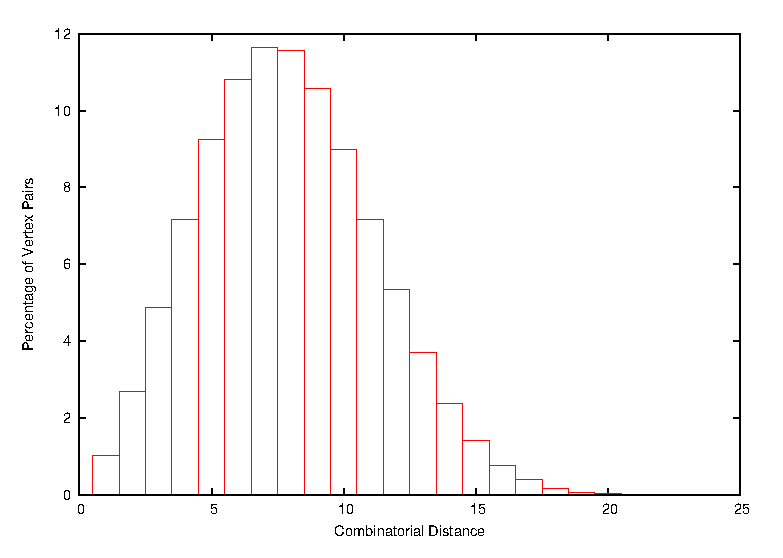
\includegraphics[width=5in]{images/connectivity_histogram.eps} 
\caption{Connectivity Histogram for a Cartesian Lattice}
\label{histogram}
\end{figure}
Another example which is analytically tractable is a tree with $n$ vertices and $n-1$ edges, where we have 
$\abs{P_i} = n-i$ for $1\le i\le n-1$. 

What can be observed from these examples is that in a Cartesian lattice the greater the size, the more diffuse  
the distribution of vertex pair distances. As the size of the spacetime complex grows, the peak shifts to greater 
combinatorial distances and also becomes much reduced. In the limit of large $n_v$, the histogram would extend 
far out along the $x$-axis with almost every distance having equal height. In a highly entwined spacetime complex, 
there would be a noticeable peak in the histogram at its left side and the vast majority of vertices would be 
only four or five hops from any other vertex.  

\subsection{Pseudomanifold Property}  

The Diaplexis library includes a method that tests whether or not the spacetime complex $\Sigma_k$ is a 
\emph{combinatorial pseudomanifold}, a much stronger property than that of being a simplicial complex. 
The three conditions that $\Sigma_k$ must meet are the non-branching requirement, dimensional homogeneity 
and being strongly connected. For $\Sigma_k$ to be non-branching means that if $\dim(\Sigma_k) = D$, then 
every $(D-1)$-simplex $\sigma\in\Sigma_k$ is a face of exactly two distinct $D$-simplices; if it is the 
face of just one $D$-simplex, then $\Sigma_k$ is a pseudomanifold-with-boundary. Dimensional homogeneity 
is the requirement that every vertex in $\Sigma_k$ must be a member of one or more $D$-simplices, i.e.\ 
$\dim(v) = D \,\,\, \forall \,\, v\in\Sigma_k$. Lastly, for $\Sigma_k$ to be strongly connected means that 
between any two $D$-simplices $\rho$ and $\tau$, we can construct a sequence of $D$-simplices 
$\sigma_1,\sigma_2,\dots,\sigma_m$ such that $\sigma_i$ and $\sigma_{i+1}$ share a face and $\sigma_1 = \rho$ 
while $\sigma_m = \tau$. Only this final property of being strongly connected requires any real work to 
be checked --- we enumerate all the $D$-simplices in $\Sigma_k$ and convert them to a graph in which 
each $D$-simplex is a vertex and there is an edge between two vertices when their respective $D$-simplices 
share a common face. If this graph is connected, then $\Sigma_k$ is strongly connected.    

\subsection{Chronotopology}

This involves a set of three methods of the \texttt{Spacetime} class:\newline
\texttt{void compute\_timestreams()}\newline
\texttt{void compute\_temporal\_vorticity()}\newline
\texttt{double compute\_temporal\_nonlinearity()}\newline
All of them operate strictly on the level of the entire active spacetime complex $\Sigma$, i.e.\ they are 
sheet-independent. The first method computes the \texttt{Vertex::past} and \texttt{Vertex::future} properties, 
which is to say the entire past and future lightcones for a given vertex. This information is needed by 
the \texttt{compute\_temporal\_nonlinearity} method as it needs to know which vertices are causal sinks (one 
whose past is non-empty but whose future is empty) and sources (vice-versa). 

The temporal vorticity $\omega_v$ of a vertex $v$ is the arithmetic mean of the cyclicity of its past 
and future causal graphs,
\begin{equation*}
\omega_v = \frac {1}{2} \left[\kappa(G_{\text{past}}) + \kappa(G_{\text{future}})\right] + \tau_v.   
\end{equation*}
An edge in a graph $G$ is said to be cyclic if the edge can be removed without disconnecting $G$ and 
the cyclicity $\kappa(G)$ is the number of cyclic edges in $G$ divided by the total number of 
edges. The second term $\tau$ in $\omega_v$ is a measure of the light cone congruence between 
spacelike-separated neighbours. We consider all neighbours $u$ of $v$ such that $\ell_{vu}^2 < 0$ and 
then calculate $J = N_v \cap N_u$. If the temporal orientation of the edges $(v,t)$ and $(u,t)$ for 
each $t\in J$ differs, then $\tau$ is increased by one; the quantity $\tau$ is finally divided 
by $\abs{J} \sqrt{-\ell_{vu}^2}$. The temporal vorticity as such measures the extent to which the causal 
structure of the vertex diverges from the classical model of a linear, acyclic flow from past to future 
and in which spacelike-separated neighbours agree in their assessment of past and future.   

The temporal nonlinearity is a global property for $\Sigma$ and the method for calculating it first determines 
the timestreams for each active vertex in $\Sigma$. For each causal source, the future-oriented causal graph 
is constructed and its cyclicity obtained, which is added to a running sum, while for each causal sink the 
past-oriented causal graph is assembled and its cyclicity added to the same running sum. This sum is then 
divided by the sum of causal sources and sinks, forming the first term in the expression for the temporal 
nonlinearity. The second term comes from looping over all active vertices in $\Sigma$ and determining which have 
a future or past lightcone containing the vertex itself, i.e.\ a causal loop, with the number of such vertices 
divided by the total number of active vertices. 

\chapter{Hyphantic Operations}

The hyphantic\footnote{From the classical Greek noun \greektext<'ufansis\latintext, which 
means ``weaving''.} operators in the Diaplexis library are the mechanism by which the spacetime 
complex's topology is modified, with each one carrying out an atomic operation of one kind or 
another on the complex: deleting or adding a 1-simplex, fusing together two vertices, inflating 
a 2-simplex into a 4-simplex and so forth. A topological transformation of arbitrary complexity 
can be achieved using a given sequence of these hyphantic operators. The hyphantic operators 
are divided into two classes, implicative (folding in) or explicative (folding out), depending on 
their effect --- those which are implicative tend to increase the topological entwinement of a given 
vertex and its neighbourhood, while explicative operators have the opposite effect, restoring an 
orthonormal Cartesian grid in the vicinity of the vertex. All of the operators are represented 
in the Diaplexis library as methods belonging to the \texttt{Spacetime} class and all of them have 
a Boolean return type, which \emph{true} indicating that the operation successfully modified the 
spacetime complex's topology. Every such method has among its arguments at least two integers, 
the first of which is the base vertex $v$, where $v = -1$ indicates that an arbitrary active 
vertex should be employed, and the second the sheet whose topology will be modified by the 
operator. 

We begin with a presentation of the implicative operators in the Diaplexis library, of which there 
are seven listed in the following chart,    
\begin{center}
\begin{tabular}{|l|l|l|}
\hline
Method Name & Symbol & Arguments \\ 
\hline \hline
fission & F & \texttt{{int,double,int}} \\
fusion & U & \texttt{{int,int}} \\
foliation & O & \texttt{{int,bool,int}} \\
perforation & P & \texttt{{int,int,int}} \\
circumvolution & V & \texttt{{int,int}} \\ 
expansion & E & \texttt{{int,double,int}} \\ 
inflation & I & \texttt{{int,double,int}} \\ 
\hline
\end{tabular}
\end{center}
The names of the operators are largely self-explanatory though their effect on the spacetime complex 
can be subtle. The \emph{fission} operator accepts as its arguments a base vertex $v$, a floating point 
argument, the density $\rho$, and finally the sheet index $n$. If $v \ge 0$, then a new vertex 
$u$ is added to the complex in the proximity of $v$, the set of neighbours of $v$ are connected to 
$u$ with probability $\rho$ and finally an edge connecting $u$ to $v$ is created. As $\rho$ varies 
over the interval $[0,1]$ the degree of topological entwinement can thus be modulated. 

The \emph{fusion} operator takes the base vertex $v$ passed as the first argument to the method and 
selects one of its neighbour vertices $u$, which is fused into $v$. All of the $n$-simplices, $n>0$, 
that contain $u$ have this replaced by the vertex $v$ so that for example all of the edges associated 
with $u$ are transferred to $v$. The \emph{foliation} operator takes the usual integer arguments of 
a base vertex $v$ and sheet $n$, while the Boolean argument determines whether or not the operator 
should act in an implicative manner. If this argument is true, then the operator selects two random 
neighbours $u$ and $w$ of $v$ such that both of them have a non-zero structural deficiency and then 
adds an edge connecting $u$ and $w$ for this sheet, if one doesn't already exist. This naturally 
also implies the creation of a 2-simplex $\{v,u,w\}$ for the sheet $n$, as well as any higher-dimensional 
simplices which depended only upon the creation of this 2-simplex to come into existence.
\begin{figure}[htp]
\centering
\label{implicative1}
\begin{tabular}{c}
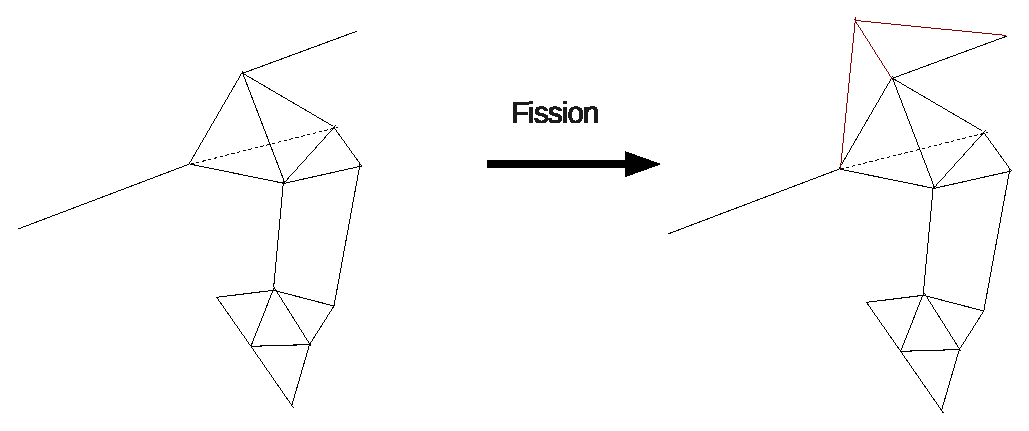
\includegraphics[width=5in]{images/fission.eps} \\
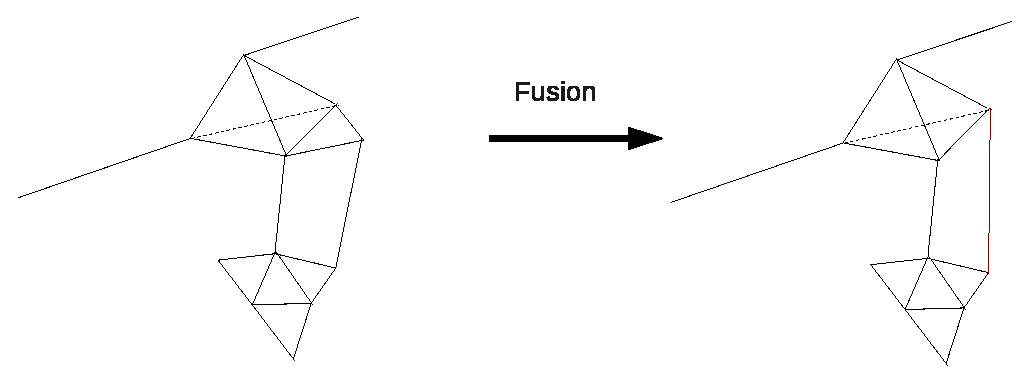
\includegraphics[width=5in]{images/fusion.eps} \\
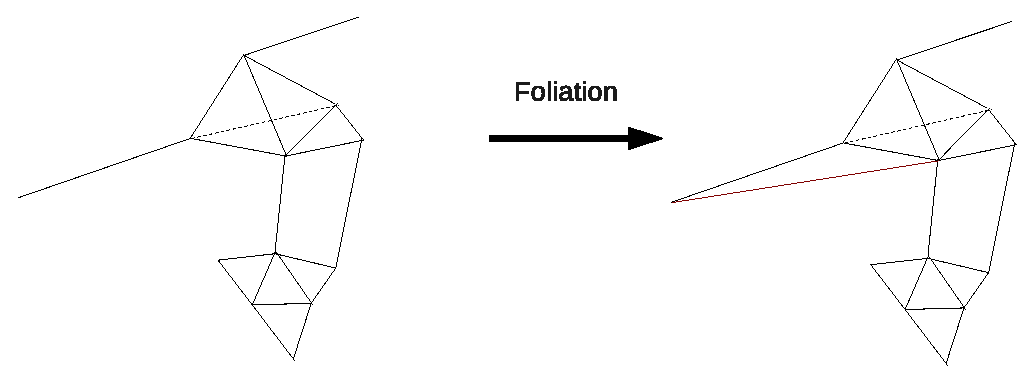
\includegraphics[width=5in]{images/foliation.eps}
\end{tabular}
\end{figure}

\begin{figure}[htp]
\centering
\label{implicative2}
\begin{tabular}{c}
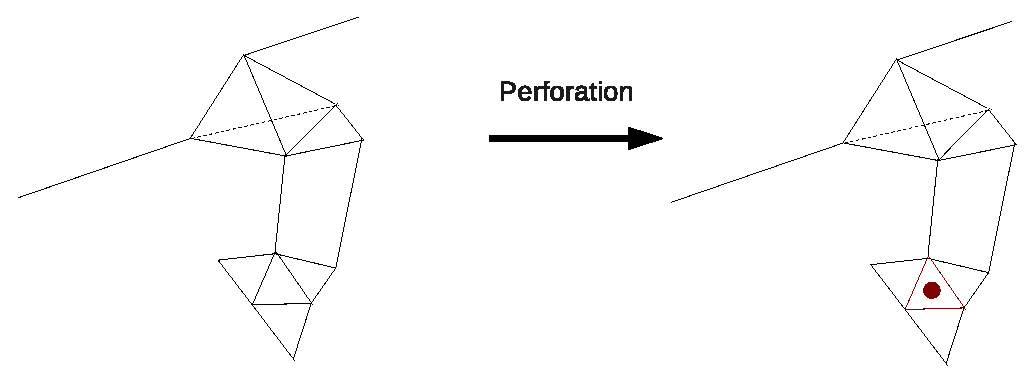
\includegraphics[width=5in]{images/perforation.eps} \\
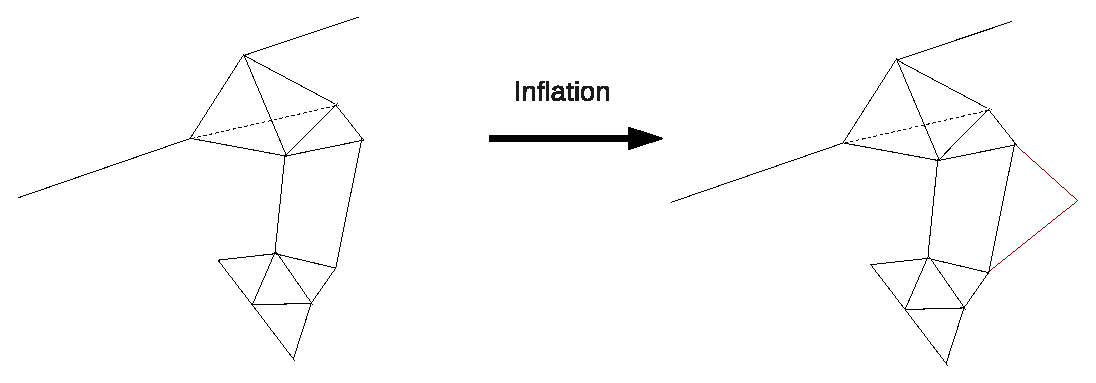
\includegraphics[width=5in]{images/inflation.eps} \\
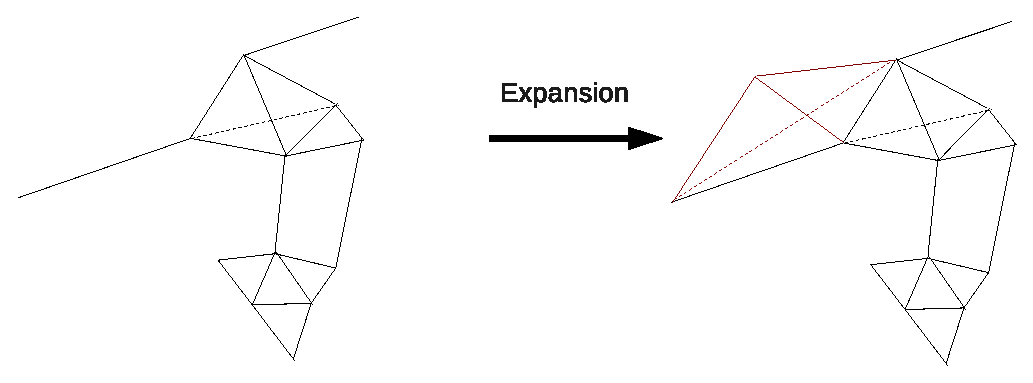
\includegraphics[width=5in]{images/expansion.eps}
\end{tabular}
\end{figure}

\begin{figure}[ht]
\centering
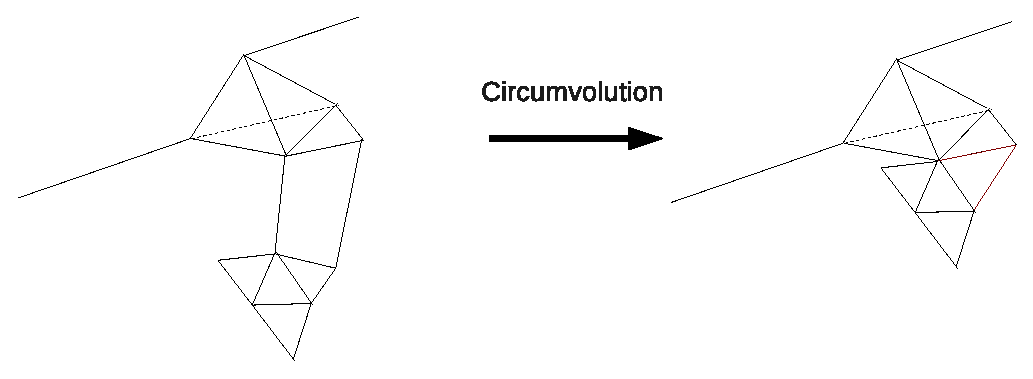
\includegraphics[width=5in]{images/circumvolution.eps}
\label{impl_circumvolution}
\end{figure}
The \emph{perforation} operator creates holes within the spacetime complex $K$, with the first argument 
$v$ and third argument $n$ having their usual sense while the second argument is important only if the 
base vertex $v = -1$.  
In this case, the second parameter $d$ specifies the dimensionality of the hole that the operator will 
attempt to create in $K$, so $2\le d\le D-1$, where $D = \dim(K,n)$. When $v \ge 0$ the dimensionality of 
the hole is chosen as a randomly between $2$ and one less than the simplicial dimension of $v$ with respect 
to the sheet $n$. The method then iterates over all $d$-simplices associated with the $n$-th sheet that 
contain $v$ (if $v\ge 0$), selecting those which have the property that each of their $1+d$ faces is also 
the face of at least one other $d$-simplex of the $n$-th sheet. Among these $d$-simplices one is then 
chosen for deletion.

The \emph{expansion} operator accepts a base vertex $v$ and as its second argument a floating 
point number which, like that for the fission operator, represents a probability $\rho \in [0,1]$, while 
the final argument is as usual the sheet $n$. In this 
case it specifies the degree to which this operator should rely on creating entirely new vertices in the 
construction of a $d$-simplex containing $v$, rather than relying on vertices that are already neighbours 
of $v$. The dimension of the new simplex is set by means of the formula 
\begin{equation}
d = \frac {D - \kappa}{1 + e^\tau} + \kappa, \qquad \tau = 25 + |\Delta_v| \label{dformula}
\end{equation}
where $\Delta_v$ is the structural deficiency of vertex $v$ and $\kappa = 1 + \dim(v,n)$. Here $D$ represents the 
maximum possible dimension of the spacetime complex, \texttt{ND}. The expansion method seeks to add a $d$-simplex 
that contains the base vertex $v$, $\rho$ percent of the neighbours of $v$ and however many new vertices are needed 
to reach the total of $1+d$ vertices. The \emph{inflation} operator works in much the same way, but starts from a 
given $m$-simplex $S$ that contains $v$ and is part of the $n$-th sheet and ``inflates'' it to a $d$-simplex, where $d$ 
is defined according to formula (\ref{dformula}). The method then assembles the set of neighbours of $v$ which are 
not part of $S$ and with probability $1-\rho$ chooses a member of this set rather than creating a new vertex to add 
the needed $d - m$ vertices for the new $d$-simplex.
     
The final implicative operator, that for \emph{circumvolution}, is also the most complicated. It selects a random 
$d$-simplex $S$ which contains the base vertex $v$ and is on the $n$-th sheet, where $d$ is also chosen randomly between 
2 and $\dim(v,n)$. We then assemble the set of $d$-simplices that are part of the $n$-th sheet and whose intersection 
with $S$ is null. From this we extract the subset of members which are at a squared distance of no more than $2.5$, 
where we define the distance between two $d$-simplices to be the largest distance between their respective vertices 
taken two at a time. If at least one such candidate exists, we then fuse it with $S$, with the mapping between the two 
sets of vertices chosen as a random shuffle of the indices.  

For the explicative operators, we have the following table analogous to that for the implicative operators.
\begin{center}
\begin{tabular}{|l|l|l|}
\hline
Method Name & Symbol & Arguments \\
\hline \hline
amputation & A & \texttt{{int,double,bool,int}} \\
fusion & U & \texttt{{int,double,int}} \\
germination & G & \texttt{{int,int}} \\
reduction & R & \texttt{{int,int}} \\
correction & C & \texttt{{int,int}} \\
contraction & N & \texttt{{int,double,int}} \\
compensation & S & \texttt{{int,bool,int}} \\
deflation & D & \texttt{{int,int}} \\
\hline
\end{tabular}
\end{center}
The \emph{contraction} operator accepts a base vertex $v$, a length threshold $\lambda$ and finally the sheet 
$n$. The method loops over all edges on the $n$-th sheet which connect the vertex $v$ and among those with a 
length greater than $\lambda$, if any exist, one is selected at random for deletion from this sheet.
\begin{figure}[ht]
\centering
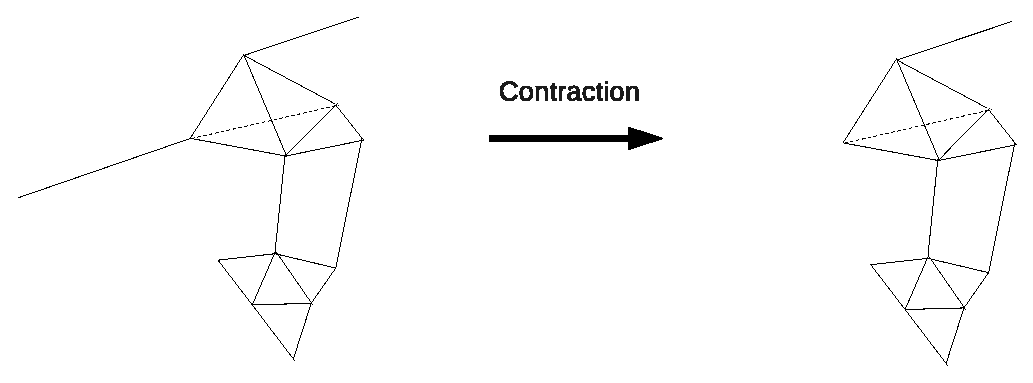
\includegraphics[width=5in]{images/contraction.eps}
\label{contraction}
\end{figure}

The \emph{deflation} operator assembles the set of $d$-simplices which contain $v$ and are part of the $n$-th 
sheet, where $d$ is a random integer drawn from the interval $[1,\dim(v,n)-1]$. If this set is non-empty then 
an element is selected for deletion. The \emph{amputation} operator has the usual first argument of a base 
vertex $v$ along with a threshold deficiency $\Delta$, a Boolean to determine if it is being called as an explicative 
operator and finally the sheet $n$. If so, then the method loops over all edges which contain $v$ and lie on the 
$n$-th sheet and if both vertices associated with this edge have a structural deficiency greater than $\Delta$ 
the vertex not equal to $v$ is added to a list of candidates. A random element of this list is chosen and is 
deleted from this sheet along with all of the $d$-simplices, $d\ge 1$ that contain it. If this renders the vertex 
chosen inactive then its energy is transferred to the vertex $v$.      
\begin{figure}[htp]
\centering
\label{explicative1}
\begin{tabular}{c}
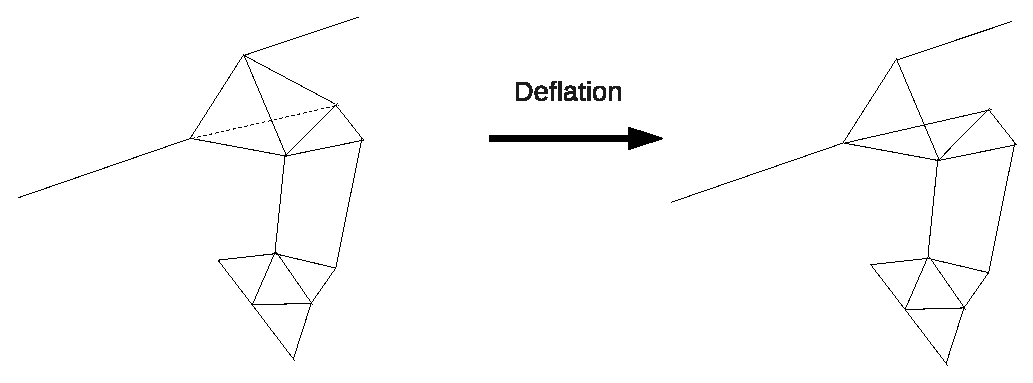
\includegraphics[width=5in]{images/deflation.eps} \\
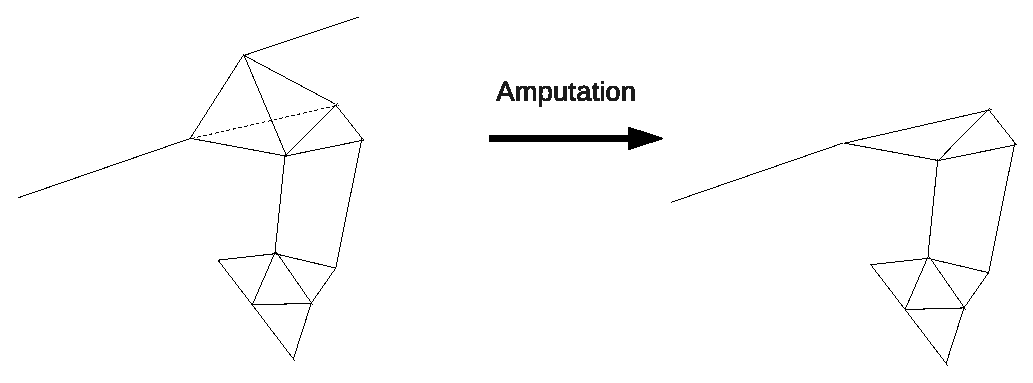
\includegraphics[width=5in]{images/amputation.eps} \\
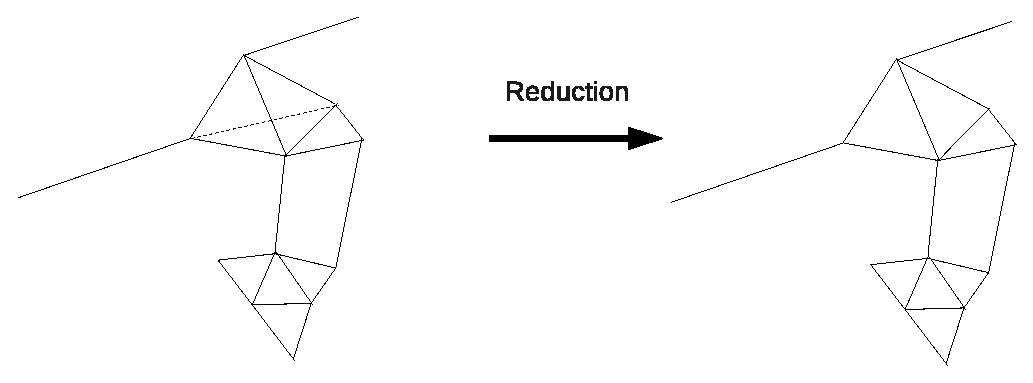
\includegraphics[width=5in]{images/reduction.eps}
\end{tabular}
\end{figure}
The \emph{reduction} operator accepts the usual integer arguments, the vertex $v$ and sheet $n$, and seeks to 
reduce the simplicial dimension $d=\dim(v,n)$ of the base vertex. The method assembles the set of all 
$d$-simplices in the spacetime complex that contain $v$ and are on the $n$-th sheet, selects one at random and 
chooses a random edge containing $v$ from this $d$-simplex's $_{d+1}C_2$ edges. 

The explicative form of the \emph{fusion} operator has as its arguments the base vertex $v$, a length threshold 
$\lambda$ and the usual final argument of the sheet $n$. This method loops over all the complex's vertices which 
lie on the $n$-th sheet and assembles the set of those which are are at a distance of less than $\lambda$ from 
$v$. A vertex $u$ is selected at random from this set and is then fused with the vertex $v$.    
\begin{figure}[htp]
\centering
\label{explicative2}
\begin{tabular}{c}
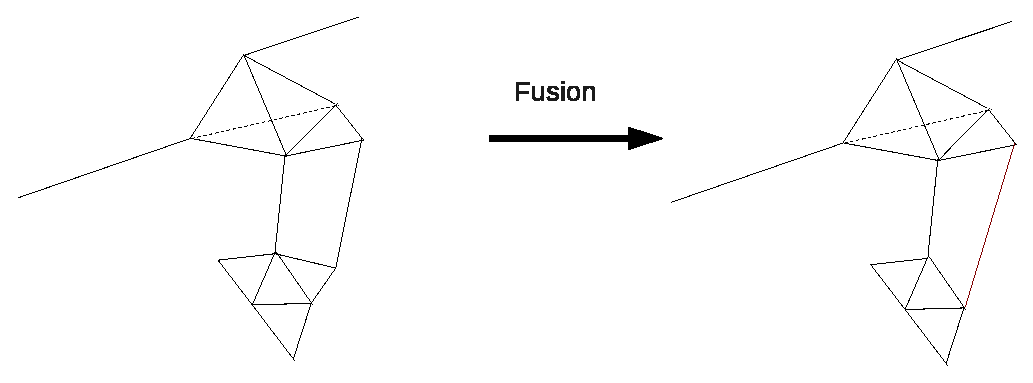
\includegraphics[width=5in]{images/fusion_x.eps} \\
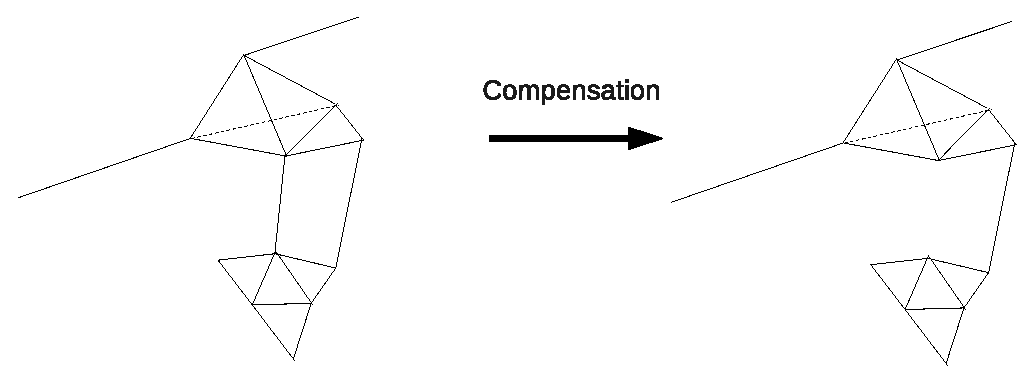
\includegraphics[width=5in]{images/compensation.eps}
\end{tabular}
\end{figure}
The \emph{compensation} operator seeks to trim the base vertex's set of neighbours so that it is more 
consistent with a Cartesian spacetime complex, through the elimination of very long or short edges, reducing 
the simplicial dimension of the base vertex to unity and ensuring that $\deg(v) = 2D$, where $D$ is the 
background dimension. The Boolean argument is used 
to determine whether the operator will seek to reduce $\dim(v,n)$ to unity (\texttt{true}) or instead to alter 
the vertex's degree (\texttt{false}). In the dimension-oriented case, the method loops over all the complex's 
edges that are part of the $n$-th sheet and contain the base vertex $v$. If the other vertex $u$ in this edge 
also satisfies the condition that $\dim(u,n) > 1$, has a structural deficiency less than zero and the edge's 
length $\ell$ satisfies $\ell < 0.9$ or $\ell > 1.1$, then the edge is added to the set of candidates for 
deletion. In the degree-oriented case, the method first determines if the base vertex $v$ has a degree with 
respect to the $n$-th sheet that is too low or too high. In the former case, the method loops over all vertices 
and assembles those which are are a distance $\delta$ from $v$ where $0.9 \le \delta \le 1.1$ and where an 
edge connecting these two vertices isn't part of the $n$-th sheet. One such vertex is selected at random and 
an edge is created. If instead $\deg(v) > 2D$, then the operator loops over all edges and assembles into a set 
those that lie on the $n$-th sheet, have a length $\ell$ outside the range $\ell \in [0.9,1.1]$ and contain 
$v$. One such edge is then selected at random for deletion.    

The \emph{correction} operator attempts to create a new vertex $w$ for the base vertex $v$ on the $n$-th 
sheet, ensuring that this new vertex is at unit distance from $v$ and any other vertices in the spacetime 
complex. The method loops over all vertices and assembles those that belong to the $n$-th sheet, have non-zero 
deficiency and are at a distance $\ell$ from $v$, where $\ell\in [1.95,2.05]$ into the set $C$. The method 
then loops over all vertices to see if any of them are at a distance in the range $[0.9,1.1]$ from those in 
$C$, if so they are put on the $n$-th sheet, if not then a vertex is created with two edges, one connecting 
it to $v$ and the other to a random member of $C$.  
\begin{figure}[htp]
\centering
\label{expl_final1}
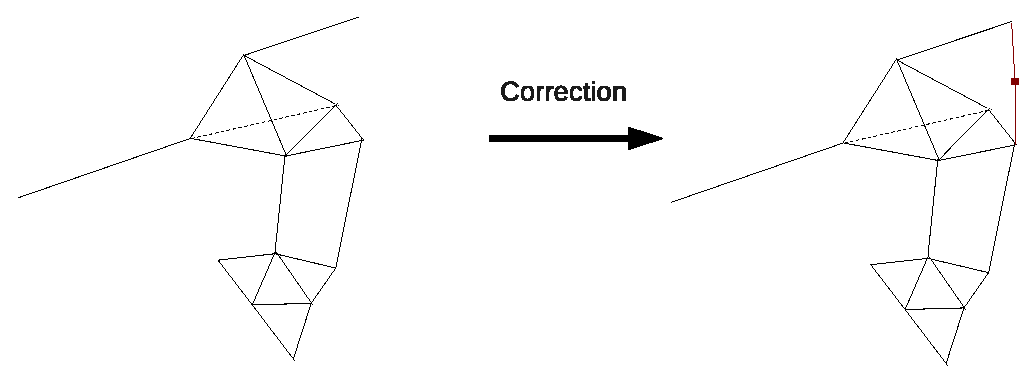
\includegraphics[width=5in]{images/correction.eps} 
\end{figure}
Lastly, the \emph{germination} operator attempts to create new vertices $w_i$ connected to the base vertex 
$v$ on the $n$-th sheet, such that the distance between $v$ and each $w_i$ is unity and the $w_i$ are all 
mutually orthogonal as well as being orthogonal to any existing edges that $v$ possesses. Naturally the 
ability to construct such additional vertices will depend on the spacetime complex's background dimension 
$D$, which in the accompanying diagrams we have assumed to be two. As this operator depends crucially on 
the ability to calculate the the angle between two edges which share a common end point it can only work 
in a spacetime complex with a non-relational geometry, i.e. one in which every vertex has a set of 
coordinates. 
\begin{figure}[htp]
\centering
\label{expl_final2}
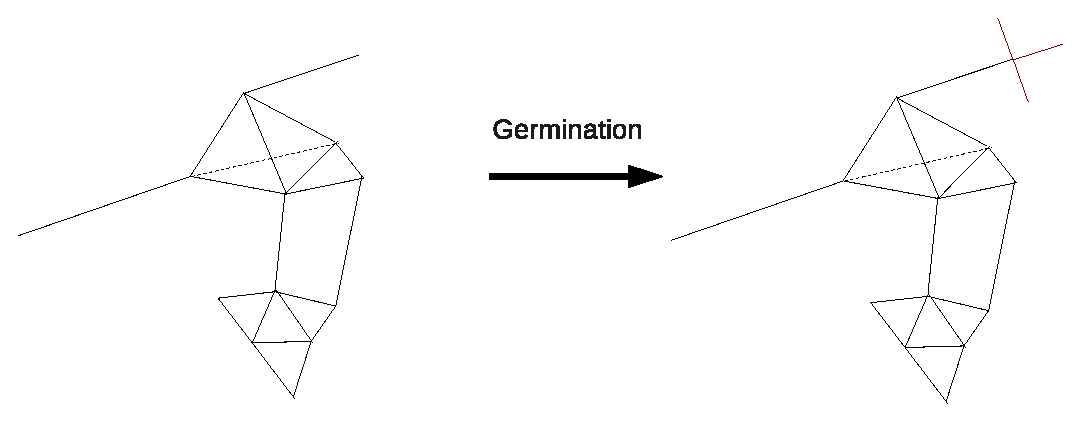
\includegraphics[width=5in]{images/germination.eps} 
\end{figure}
 
The manner in which the Diaplexis library decides which operator to apply in a given context depends on 
several factors. The \texttt{Spacetime} class has two methods, one to generate the particular implicative 
(\texttt{implication}) and the other to do the same for explicative operators (\texttt{explication}). Each 
method uses a set of probabilities as well as the number of elapsed iterations to determine which 
operator should be returned. 

When the \texttt{Spacetime::hyphansis} method is called with a given sheet $n$ as its argument, it first 
loops over the complete set of spacetime vertices and places those which belong to the $n$-th sheet
and which have a non-zero deficiency in a vector of candidates for hyphansis, sorted by the magnitude of 
the deficiency from highest to lowest. If this vector is empty the method returns immediately while in the 
case where there is only one candidate vertex and its deficiency is negative, the method applies the 
expansion operator and then returns.

The method loops over the elements of the vector of candidate vertices, checking to verify that the vertex 
$v$ is active (as a candidate vertex may have been removed from this sheet by an earlier hyphantic 
operation) and based on the sign of its structural deficiency $\delta_v$ generates an implicative 
(deficiency less than zero) or explicative operator. In the case of an implicative operator, the 
probabilities are as follows:
\begin{center}
\begin{tabular}{|l|l|l|l|}
\hline
Operator & Argument(s) & Probability (Stage 1) & Probability (Stage 2)\\ 
\hline \hline
F & 0.4 & 30\% & 10\% \\
U &     & 15\% & 10\% \\
O & \texttt{true} & 15\% & 20\% \\
P & 0    & 3.3\% & 25\% \\
V &      & 6.7\% & 25\% \\ 
E & 0.15 & 15\%  & 6.7\% \\ 
I & 0.25 & 15\%  & 3.3\% \\ 
\hline
\end{tabular}
\end{center}
where the initial stage is during the initial fifty relaxation steps for the spacetime complex. As for the 
generation of the explicative operators, the schema employed is considerably more involved. If the vertex 
in question has a simplicial dimension greater than one, then with probability $\delta_v/10$ the deflation 
operator is called, otherwise the reduction operator. Assuming instead that $\dim(v) = 1$, which 
explicative operator is called depends on whether the simulation is in the initial or secondary stage. 
If the simulation is still in the first 
stage, then with probability $0.35 + 1/(1+k/2)$ where $k$ is the number of elapsed iterations the 
compensation operator is called, alternatively if $k \le 10$ the correction operator is called and if 
$k>10$, then the correction and amputation operators are called with equal likelihood. If instead the 
simulation has entered the second stage, the operators \texttt{{C,S,N,U}} are called with equal likelihood. 
Finally, when $\dim(v) = 1$ and the reduction operator was applied without success, the contraction and 
fusion operators are attemped with equal probability; if the selected operator(s) had no success, a last  
attempt is made to apply the compensation operator. The extra arguments employed in all such cases are, 
\begin{center}
\begin{tabular}{|l|l|}
\hline
Operator & Argument(s) \\
\hline \hline
S & \texttt{false} \\
G &     \\
A & \texttt{{10.0,true}} \\
R &    \\
C &    \\
D &    \\
U & 0.5\\
N & 1.2\\
\hline
\end{tabular}
\end{center}   
Once the hyphantic operator has been applied, if its action was successful then the regularization method 
is called for this sheet, the operation is logged and the count of successful hyphantic operations is 
incremented by one. When this number exceeds 10\% of the active vertices for this sheet, the main hyphantic 
loop is exited and the method call terminates, ending hyphansis for this particular sheet. When the 
hyphansis step takes place, every active sheet is called in random order.  
  
\chapter{Geometry Solvers}

The software library comes with five different geometry solvers: mechanical (effective force), 
evolutionary, simplex method, simulated annealing and minimal (random) solvers. The geometry stage in 
the relaxation process differs from that of hyphansis because the geometry of the spacetime complex is 
universal, that is it doesn't depend on the particular sheet. The coordinates of a vertex $v$ or the 
length of an edge $e_{uv}$ are the same for all sheets, what varies between the sheets is the topology 
of the spacetime complex. For this reason the geometrical modifications of the spacetime complex take 
place within the method \texttt{Spacetime::global\_operations}, along with the energy diffusion and the 
calculation of global terms in the structure equation. 

\section{Minimal Solver}

By default the minimal solver is used, whose algorithm is a brute force random search: 
a list of candidate vertices is assembled --- those which are active, have a non-zero 
structural deficiency and all of whose neighbours also have a non-zero structural 
deficiency --- from which a vertex is selected at random. Each coordinate of the vertex 
is multiplied by a different normal variate $N(1,\sigma)$ with standard deviation
\begin{equation*} 
\sigma = \min\left(\frac {1}{2},\frac{\Delta_G}{10}\right)
\end{equation*}
where $\Delta_G$ is the vertex's geometric deficiency. The spacetime's structural deficiency 
is then recalculated; if it is lower, the change is accepted, otherwise it is rejected. After 
\texttt{SolverIterations} such steps have been carried out, the solver quits and control is 
returned for another round of topological hyphansis.  

\section{Evolutionary Solver}

The evolutionary solver creates a population of spacetime geometries of size equal to the parameter 
\texttt{pool\_size}. Each geometry is initialized with the current spacetime geometry along with a random 
jitter, in which 15\% of the geometry variables are modified additively. The structural deficiency 
of each member of the pool is calculated. Next we enter the evolutionary loop, which is executed 
\texttt{ngenerations} times. At each iteration, each member of the pool creates one child with which it 
shares the same geometry, a single element of this child's geometry which is associated with a vertex 
who geometric deficiency is non-zero is then mutated and its structural deficiency is calculated. To 
determine which of total pool of \texttt{2*pool\_size} individuals will survive to the next iteration, 
we carry out a series of stochastic tournaments. For each individual $q$, we conduct \texttt{njousts} 
contents with other randomly selected individuals $p$ in the population. We compute 
\begin{equation*}
\rho = \frac {1}{2}\left[1 + \tanh(\sigma_p - \sigma_q)\right]
\end{equation*}
where $\sigma_i$ is the structural deficiency of the $i$-th individual; if $\rho$ is greater than a 
uniform random variate on $[0,1)$, we say that $q$ has won the joust. We then choose those individuals 
which won \texttt{njousts}, \texttt{njousts-1}, \texttt{njousts-2} etc.\ tournaments, until we have 
obtained the needed \texttt{pool\_size} elements. When the generations have run their course, the 
individual with the lowest structural deficiency has its geometry written to that of the spacetime 
complex.
  
\section{Simulated Annealing Solver}

In this method we first need to calculate the melting temperature of the spacetime complex's geometry, 
that is the value of $T$ such that between 80\% and 85\% of the changes made to the spacetime geometry 
are accepted using the Metropolis criterion, $\exp[-(E_2 - E_1)/T]$ where $E_1 < E_2$ and $E_1$ and 
$E_2$ are the structural deficiency before and and after the random geometry change. To do this we 
begin with $T=100$ and enter a loop inside of which one thousand Metropolis steps are performed. The 
acceptance percentage is calculated and the temperature is multiplied by 1.1 if it is less than 80\% 
or multiplied by 0.9 if it is more than 85\%. As with the evolutionary solver, only those vertices 
with a non-zero geometric deficiency have their geometry modified.   

Once the melting temperature of the spacetime geometry has been determined, the simulated annealing 
process properly speaking begins from this temperature $T_i$. A loop is performed over the number of 
annealing steps, with the temperature multiplied by 0.9 at each iteration. In the interior of this 
primary loop is a do-while loop which is responsible for thermalizing the spacetime geometry at the 
current temperature. This is done by having a loop perform \texttt{thermal\_sweep} Metropolis steps 
on the geometry, calculating the standard deviation of the structural deficiency since the last 
temperature change and checking to see if it is lower than the thermalization threshold. Throughout 
the entire simulation we keep track of which geometry has the lowest overall structural deficiency 
and upon finishing the annealing schedule this geometry is applied to the spacetime complex.    
 
\section{Mechanical Solver}

This solver is based on an effective force algorithm such as are used to calculate aesthetically 
pleasing geometric embeddings of abstract graphs. It uses a mechanical model of the graph, in 
which edges are represented as springs governed by Hooke's law in conjunction with a universal 
inter-vertex repulsion and a small dissipative factor. The graph is then subjected to Newton's 
laws of motion from the geometry's initial state with zero initial velocity,
\begin{equation}
\frac {d^2\mathbf{x}_i}{dt^2} = k \frac {d\mathbf{x}_i}{dt} + \mathbf{F}_i(\mathbf{x})
\end{equation} 
where 
\begin{equation}
\mathbf{F}_i = R \sum_{j=1}^N \frac {\mathbf{x}_i - \mathbf{x}_j}{\norm{\mathbf{x}_i - \mathbf{x}_j}^2} + 
            \omega \sum_{e_{ij}\in N_i} (\mathbf{x}_i - \mathbf{x}_j) 
\end{equation}
and $\mathbf{x}_i(0)$ is set to the current spacetime geometry while $\dot{\mathbf{x}}_i(0) = 0$ for all $1\le i\le 
N$ and $N$ of course is the number of active vertices in the spacetime. This algorithm only makes sense in 
the context of an absolute model for the spacetime geometry and we assume that the geometric dimensionality 
of the vertices is uniformly equal to the background dimension $D$. The user can specify the value of the 
damping constant $k$, the repulsion constant $R$ and the spring constant $\omega$, as well as the type of 
integration engine used (forward Euler or fourth-order Runge-Kutta), the step size and the maximum number 
of integration steps. The numerical integration of the mechanical system is terminated when this maximum 
number of steps is reached or the value of $\norm{\dot{\mathbf{x}}}(t_n)$ is lower than the geometry cutoff. 
In order to account for the influence of a vertex's energy on its geometry, the true repulsion $R_{\mbox{true}}$ 
between two vertices $v_i$ and $v_j$ is defined to be 
\begin{equation*}
R_{\mbox{true}} = \frac {R}{1 + (E_i + E_j)/2}  
\end{equation*}
where $E_i$ is the energy of $v_i$.

The user can also choose to perform a conjugate gradient minimization (using the Polak-Ribi\`ere variant of 
the method) of the spacetime's abnormality once the integration of the mechanical system has converged. This 
minimization only works with the abnormality because the obliquity term in the formula for the geometric 
deficiency is non-analytic. The function being minimized then is simply 
\begin{equation}
F(x) = \sum_{i=1}^N \sum_{j=1+i}^N (\ell_{ij} - \norm{x_i - x_j})^2
\end{equation}
where $\ell_{ij} = (1+(E_i + E_j)/2)^{-1}$ is the optimal length for the edge, given the average energy of 
the two vertices, unless the edge $(v_i,v_j)$ is ``flexible''. These are the edges which connect a zero 
energy vertex that is a neighbour of a positive energy vertex to other zero energy vertices and they need 
to be able to expand in size to prevent a single positive energy vertex from perturbing a significant 
region of the spacetime complex from being orthonormal. These flexible edges contribute a term of the 
form $(\Lambda - \norm{x_i - x_j})^2$ when $\norm{x_i - x_j} > \Lambda$ and zero otherwise, where $\Lambda$ 
is the \texttt{EdgeFlexibilityThreshold} run-time parameter.
  
The conjugate gradient method applied to the nonlinear function $F(x)$ begins with the observation that 
the gradient $\nabla_x F = 0$ when $F$ is minimal. As the gradient indicates the direction of greatest 
increase, the minimization method moves in the opposite direction $\Delta x_0 = -\nabla_x F(x_0)$, performing 
an iterative line search $\alpha_0 = \min\limits_{\alpha} F(x_0 + \alpha \Delta x_0)$ then calculating 
$x_1 = x_0 + \alpha_0 \Delta x_0$. For a general iteration we have the algorithm,\newline
1) Calculate the direction of steepest descent, $\Delta x_n = -\nabla_x F(x_n)$\newline
2) Compute $\beta_n$ according to the formula,
\begin{equation*}
\beta_n = \frac {\Delta x_n^T \left(\Delta x_n - \Delta x_{n-1}\right)}{\Delta x_{n-1}^T \Delta x_{n-1}}
\end{equation*}
3) Calculate $s_n = \Delta x_n + \beta_n s_{n-1}$\newline
4) Do the line search, $\alpha_n = \min\limits_{\alpha} F(x_n + \alpha s_n)$\newline
5) Update the spacetime geometry, $x_{n+1} = x_n + \alpha_n s_n$\newline
The only user-controlled parameters concern the maximum number of iterations to use for the line search that 
defines $\alpha$ and the maximum number of overall conjugate gradient iterations. The algorithm stops when 
this latter number is reached or the structural deficiency falls below the geometry cutoff.  

\section{Simplex Solver}

This algorithm is based on the Nelder-Mead method in which we construct an initial $k$-simplex $S$, 
where $k$ is equal to the dimension of the spacetime complex's geometry $N_G$. In the relational case, 
this is the number of $1$-simplices in the spacetime, while for an absolute geometry we have
\begin{equation*}
N_G = \sum_{i=1}^N \max(\dim(v_i),D)
\end{equation*}
where $D$ is the background dimension and $N$ the number of vertices in the spacetime complex $\Sigma$. 
We assume that $\dim(v)=0$ if and only if $v$ is an inactive vertex. Each vertex of $S$ is obtained by 
making a Gaussian modification of one element of the original geometry of the spacetime complex and we 
calculate the structural deficiency associated with each of these vertices of $S$, which are then sorted 
in ascending order.   

The main body of this optimizer is a do-while loop which is exited when the lowest structural 
deficiency value of any vertex in $S$ is less than the geometric threshold or $10N_G$ iterations of 
the loop have been performed.At each iteration, the centroid $v_c$ of $S$ is calculated and its 
reflection,
\begin{equation*}
v_\alpha = (1+\alpha) v_c - \alpha v_w 
\end{equation*}
where $v_w$ is the $S$ vertex with the highest structural deficiency. We calculate the structural 
deficiency $E_\alpha$ of $v_\alpha$ and then choose which transformation to apply to $S$ based on the 
value of $E_\alpha$. If $E_\alpha$ is lower than any existing vertex of $S$, we try an expansion, creating 
a second vertex of $S$ defined by $v_\gamma = (1+\alpha\gamma) v_c - \alpha\gamma v_w$ and calculate its 
structural deficiency, $E_\gamma$. If $E_\gamma < E_\alpha$ then we set $v_w = v_\gamma$, otherwise $v_w = 
v_\alpha$. If instead $E_\alpha$ lies between the lowest and second highest structural deficiency values 
of $S$, we set $v_w = v_\alpha$. If $E_\alpha$ is greater than the second highest structural deficiency 
value but lower than $E_w$ (the highest), we compute the hypothetical vertex $v_\rho = (1+\alpha\rho) 
v_c - \alpha\rho v_w$ and calculate its structural deficiency, $E_\rho$. If $E_\rho < E_\alpha$, we set 
$v_w = v_\rho$, otherwise we modify the value of all the vertices of $S$ except the one with the lowest 
structural deficiency, according to the formula $v_i = v_b + \sigma (v_i - v_b)$ (where $v_b$ is the 
vertex corresponding to the best structural deficiency value), then recalculate the structural deficiency 
for all of these modified vertices. Finally, if $E_\alpha > E_w$, then we perform an internal contraction 
of $S$, obtaining the new vertex $v_\rho' = (1-\rho) v_c + \rho v_w$, whose structural deficiency 
$E_\rho'$ we compute and if $E_\rho' < E_w$, we set $v_w = v_\rho'$. If instead $E_\rho' \ge E_w$, we apply 
the same approach as mentioned above to modify all of the $N_G$ vertices of $S$ with a non-optimal 
structural deficiency, employing the same formula of $v_i = v_b + \sigma (v_i - v_b)$. 

The transformations discussed in the preceding paragraph explain the constraints on the parameter 
values, namely $\alpha > 0$, $0 < \rho < 1$, $0 < \sigma < 1$ and $\gamma > \max(1,\alpha)$, and 
which correspond to the following parameter file fields: 
\begin{center}
\begin{tabular}{|c|c|}
\hline
\emph{Parameter Name} & \emph{Variable} \\ \hline
Reflection Coefficient & $\alpha$ \\ \hline
Expansion Coefficient & $\gamma$ \\ \hline
Contraction Coefficient & $\rho$ \\ \hline
Shrinkage Coefficient & $\sigma$ \\ \hline
\end{tabular}
\end{center}    
    
\chapter{File Formats}

This chapter discusses the format of the three kinds of disk files used by the Diaplexis library, the 
text-based log and incastrature\footnote{From the Latin noun \emph{incastratura, -ae} which means an 
encasement or nesting inside one another.} files and the binary state file used for checkpointing the 
program execution. The incastrature file is only produced at the end of the relaxation process, either 
because the spacetime complex has converged or because the maximum number of iterations has been exceeded. 
The checkpoint file is produced for the initial configuration as well as the final relaxation step, in 
addition to the frequency specified by the parameter \texttt{CheckpointFrequency}, assuming that the 
parameter \texttt{Checkpoint} has been set to true. 

\section{The Log File}

This is an XML file that is created at program start-up (during the call to the \texttt{initialize} method 
of the \texttt{Spacetime} class) and updated at each relaxation step, as the final component of the global 
operations for that iteration. A post-amble is written to the log file when the program execution is complete. 
During the first call to the method \texttt{Spacetime::write\_log}, fields containing global information 
about this run will be written to the file, such as the branch of the Diaplexis library used (NTL or STL), 
the hostname of the machine on which it is running, the date and time of the program execution and the 
value of both the compile-time parameters (see Table (\ref{ct_parms})) and run-time parameters (see 
Tables (\ref{rt_parms1}) and (\ref{rt_parms2})). The XML tree structure has the following form
\begin{center}
\Tree [.LogFile CompileTimeParameters [.RunTimeParameters Global Geometry ] [.RelaxationStep Sheet ] ]  
\end{center}
in which we neglect all of the leaves and simply consider the branch structure. At each iteration, an 
additional instance of a \texttt{RelaxationStep} is added, with each such step consisting of multiple 
instances of \texttt{Sheet}, one for each sheet in the polycosmic spacetime complex, along with a set of 
global statistics for the ``global'' simplicial complex consisting of all active elements (i.e.\ which 
belong to at least one sheet). The data that is written to the log file for a given sheet, including 
the global sheet, can be seen in Table (\ref{log-sheet}). For the global sheet the quantities 
\texttt{Iteration} (integer) and \texttt{StructuralDeficiency} (double) are prepended, while for an 
element of the codex array the \texttt{Index} (integer) and \texttt{State} (a Boolean) are prepended 
and the \texttt{HyphanticSequence} is appended. 
\begin{table}
\centering
\begin{tabular}{|c|c|}
\hline
\emph{Name} & \emph{Type} \\ \hline
Pseudomanifold & \texttt{bool} \\ \hline
Boundary & \texttt{bool} \\ \hline
Orientable & \texttt{bool} \\ \hline 
Cyclomaticity & \texttt{int} \\ \hline
ActiveVertices & \texttt{int} \\ \hline
SourceVertices & \texttt{int} \\ \hline
SinkVertices & \texttt{int} \\ \hline
ActiveEdges & \texttt{int} \\ \hline
TimelikeEdges & \texttt{int} \\ \hline
SapcelikeEdges & \texttt{int} \\ \hline
NullEdges & \texttt{int} \\ \hline
CyclicEdges & \texttt{int} \\ \hline
MinArcLength & \texttt{double} \\ \hline
AvgArcLength & \texttt{double} \\ \hline
MaxArcLength & \texttt{double} \\ \hline
MinVertexDegree & \texttt{int} \\ \hline
AvgVertexDegree & \texttt{double} \\ \hline
MaxVertexDegree & \texttt{int} \\ \hline
MinVertexDimension & \texttt{int} \\ \hline
AvgVertexDimension & \texttt{double} \\ \hline
MaxVertexDimension & \texttt{int} \\ \hline
TotalEnergy  & \texttt{double} \\ \hline
MinVertexEnergy & \texttt{double} \\ \hline
AvgVertexEnergy & \texttt{double} \\ \hline
MaxVertexEnergy & \texttt{double} \\ \hline
AtemporalVertices & \texttt{int} \\ \hline
ChiralVertices & \texttt{int} \\ \hline
EulerCharacteristic & \texttt{int} \\ \hline
\end{tabular}
\caption{Logfile Sheet Properties}
\label{log-sheet}
\end{table}

At the end of execution two final fields are added to the file's preamble, specifying the time and date 
that execution finished as well as whether or not the simulation converged; a false value means that the 
program came to an end because the maximum number of relaxation steps was attained. 
   
\section{The State File}

The state file is a binary file format that contains all the data necessary to restart the relaxation 
process from a given iteration. The file begins with a header that specifies the values of all of the 
global parameters used in the simulation:
\begin{center}
\begin{tabular}{|c|c|}
\hline 
\emph{Name} & \emph{Type} \\ \hline
Maximum Simplicial & \texttt{int}\\
Dimension & \\ \hline
Number of Atomic & \texttt{int} \\
Propositions per Clause & \\ \hline
Background Dimension & \texttt{int} \\ \hline
Relational Geometry & \texttt{int} \\
(1 = true, 0 = false) & \\ \hline
Dimensional Uniformity & \texttt{int} \\ 
(1 = flat, 0 = non-flat) & \\ \hline
Topological Radius & \texttt{int} \\ \hline 
Polycosmic Ramosity & \texttt{double} \\ \hline 
Machine Epsilon  & \texttt{double} \\ \hline
Initial Temperature for & \texttt{double} \\ 
Permutation Annealing & \\ \hline
Thermal Decay Rate for & \texttt{double} \\ 
Permutation Annealing & \\ \hline 
\end{tabular} 
\end{center}
As these are all compile-time constants, when the a spacetime state file is read the Diaplexis library will 
verify that the current values for these constants are the same as those found in the file.   

The next element of a state file is the set of run-time parameters that control program execution and 
which are stored in the same order as they appear in Tables (\ref{rt_parms1}) and (\ref{rt_parms2}), 
with the exception of the \texttt{Euclidean} and \texttt{InputFile} parameters which are unnecessary 
in this context.

The principal body of the state file consists of the serialization of the essential properties of the 
\texttt{Spacetime} class, written to the file in the following manner: the geometry, vertices, $k$-simplices in 
ascending order of dimensionality from $1$ to \texttt{ND}, the integral homology groups $H_k(\Sigma,
\mathbb{Z})$ for $0\le k \le \dim(\Sigma)$, the fundamental group $\pi_1(\Sigma)$ and finally the codex 
of sheets that exist at the moment the state file is written to disk.

The last element of the state file is the anterior spacetime state --- the curren values for the 
topological, geometric and energy delta are written to the file and then the contents of the 
\texttt{Spacetime::anterior} property, first the vertices and then the higher-dimensional simplices 
in ascending dimensional order. When the a state file is read in, the index tables for the spacetime 
itself as well as its anterior state is regenerated from scratch.  
 
\section{The Incastrature File}

This is a plain text file that follows the DOT format for use with the GraphViz software and contains 
a complete description of the incidence structure of the spacetime complex, which is to say its 
combinatorial topology. Using GraphViz, the file can be converted into a PDF of the Hasse diagram 
for the spacetime topology, viewed as a partially-ordered set (poset). The format of the file is 
fairly simple, with the initial line and final lines establishing the framework for a directed graph 
(digraph) $G$, with a single line in the body of $G$ for each of the $(1+k)$ faces of every $k$-simplex 
in the spacetime complex. Thus a complex consisting of the single 2-simplex $\{a,b,c\}$ and its implied 
sub-simplices would lead to the following incastrature file,
\begin{verbatim}
digraph G {
"a:b:c" -> "a:b";
"a:b:c" -> "a:c";
"a:b:c" -> "b:c";
"a:b" -> "a";
"a:b" -> "b";
"a:c" -> "a";
"a:c" -> "c";
"b:c" -> "b";
"b:c" -> "c";
"a" -> "NULL";
"b" -> "NULL";
"c" -> "NULL";
}
\end{verbatim} 
When processed through the GraphViz software this would lead to the Hasse diagram Figure~\ref{hasse}, 
which in this simple case is obviously uninteresting but for a spacetime complex with a richer incidence 
structure could be a useful way of visualizing the nature of the topological entwinement that exists 
among the various $k$-simplices. 
\begin{figure}[htp]
\centering
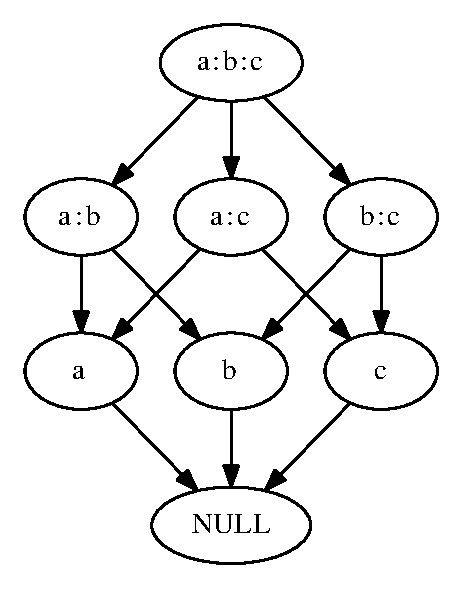
\includegraphics[width=5in]{images/scomplex.eps}
\caption{Hasse Diagram for the Simplicial Complex $\{a,b,c\}$}
\label{hasse} 
\end{figure}
The GraphViz software is available at no cost for the Linux, OS X and Windows platforms and users of the 
Diaplexis library are encouraged to download it from the \texttt{www.graphviz.org} site. 
\begin{thebibliography}{99}
\bibitem{Edelsbrunner:2001} Edelsbrunner, Herbert, \emph{Geometry and Topology for Mesh Generation}. Cambridge (UK): 
Cambridge University Press, 2001
\bibitem{Edelsbrunner:2010} Edelsbrunner, Herbert and Harer, John, \emph{Computational Topology: An Introduction}. 
Providence (RI): AMS Press, 2010
\bibitem{Godsil} Godsil, Chris and Royle, Gordon, \emph{Algebraic Graph Theory}. New York (NY): Springer, 2001
\bibitem{Hungerford} Hungerford, Thomas, \emph{Algebra}. New York (NY): Springer, 1989
\bibitem{Munkres} Munkres, James, \emph{Elements of Algebraic Topology}. Boulder (CO): Westview Press, 1996
\bibitem{Nakahara} Nakahara, Mikio, \emph{Geometry, Topology and Physics}, 2nd Edition. New York (NY): Taylor and 
Francis, 2003 
\bibitem{Zomorodian} Zomorodian, Afra, \emph{Topology for Computing}. Cambridge (UK): Cambridge University Press, 2005
\end{thebibliography}
\end{document}
